%%%%%%%%%%%%%%%%%%%%%%%%%%%%%%%%%%%%%%
% This is the name of the style file.
%%%%%%%%%%%%%%%%%%%%%%%%%%%%%%%%%%%%%%
%
% phd  -> for a PhD dissertation
% ms   -> for an MS thesis
% If both phd and ms are used then phd will overide.  If none are used,
% then ms will be active by default.
%
% cpyr -> generate a copyright page
% lof  -> generate List of Figures
% lot  -> generate List of Tables
\documentclass[ms,cpyr,lof,lot]{uathesis}
%\documentclass[ms]{uathesis}
%
%%%%%%%%%%%%%%%%%%%%%%%%%%%%%%%%
% List of any packages you use.
%%%%%%%%%%%%%%%%%%%%%%%%%%%%%%%%
%
\usepackage{amsmath}
\usepackage{amssymb}
\usepackage{graphicx}

\usepackage{listings}
\usepackage{color}
\usepackage{setspace}
\usepackage{subcaption}
\usepackage[table]{xcolor}
\usepackage{textcomp}

%
%%%%%%%%%%%%%%%%%%%%%%%%%%%%%%%%%%
% List of definitions you define.
%%%%%%%%%%%%%%%%%%%%%%%%%%%%%%%%%%
%
\def\ds{\displaystyle}
\def\E{\epsilon}
\def\eps{\varepsilon}
\definecolor{lightgray}{gray}{0.9}
%

\title{Deformation of carbon nanotube fibers interacting with rigid substrates}
\author{Andrew Robert Marmaduke}
\conferraldate{May}{2015}

%The following commands specify the names and titles of people that
%will appear on the signature page.
%
%These four will always be needed.
\advisor{Dr. Dimitry Golovaty}
\chair{Dr. Timothy Norfolk}
\collegedean{Dr. Chand Midha}
\gradschdean{Dr. George R. Newkome}
%
%For a PhD dissertation, specify a coadvisor and three committee
%members, or four committee members only.  For an MS thesis use either
%one coadvisor or one faculty reader, not both.
%
%Typical commands for a PhD dissertation (uncomment only 4).
%\coadvisor{Dr. J Patrick Wilber}
%\committee{Name of 1st Comm Member}
%\committee{Name of 2nd Comm Member}
%\committee{Name of 3rd Comm Member}
%\committee{Name of 4th Comm Member}
%
%Typical commands for an MS thesis (uncomment only 1).
\coadvisor{Dr. J Patrick Wilber}
%\facreader{Name of Fac Reader}
%\facreader{Name of Fac Reader}

\begin{document}

\maketitle
\chapter{INTRODUCTION} \label{chap:one}

\section{Graphene and carbon nanotubes}
	
	Graphene is a configuration of covalently bonded carbon atoms arranged in a two-dimensional hexagonal lattice. It is known to be a structural component to graphite, carbon nanotubes, and other materials. However, the existence of stable graphene sheets was only speculative, until they were isolated experimentally in 2004 \cite{Novoselov2004}. Graphene has many potential applications, primarily because of the high Young's modulus, room temperature electron mobility, thermal conductivity, optical absorption, gas impermeability, etc \cite{Novoselov2012}. Recently developed novel transistors \cite{Lin2010} and composite materials for solar cells \cite{Wang2013} emphasize the future promise of graphene. Mass production of an acceptable quality of graphene is, however, still in its infancy, and with it so are industrial applications \cite{Novoselov2012}.
	
	\begin{figure}
		\begin{center}
			\def\svgwidth{.75\columnwidth}
			\input{./old_fig/Chirality.eps_tex}
		\end{center}		
		\caption{A graphene sheet with possible choices of a chiral vector $\mbox{C}_{\textbf{v}}$.
		\label{fig:GrapheneCat}}
	\end{figure}	
	
	Carbon nanotubes were first identified in 1950's although they were brought to the attention of the wider scientific community in 1991 \cite{Iijima1991}. A carbon nanotube (CNT) can conceptually be thought of as an appropriately rolled graphene lattice (see Fig.~\ref{fig:GrapheneCat}). CNTs are categorized by their chirality and the number of encasing shells. A CNT is called a single-walled carbon nanotube (SWCNT) if there is only one cylindrical structure with no additional interior or exterior CNTs, a double-walled carbon nanotube (DWCNT) if there is exactly two concentric CNTs, or a multi-walled carbon nanotube (MWCNT) if there are more than two. Chirality of a CNT is categorized by a vector on a graphene sheet. The basis for this vector is shown on Fig.~\ref{fig:GrapheneCat}, $a_1$ and $a_2$, which forces head and tail points to lie on vertices of a hexagon. A CNT is then formed by rolling the graphene sheet along the vector, $\mbox{C}_{\textbf{v}}$, until the head and tail points meet. In this way $\mbox{C}_{\textbf{v}}$ determines the circumference of the CNT and an orthogonal vector T is the tube axis. The tail is usually taken as a reference or origin point, and then chirality is determined by the position of the head. A CNT is called armchair if along the tube axis the hexagon structure repeats uniformly (see Fig.~\ref{subfig:Armchair}), zigzag if the hexagon structure alternates (see Fig.~\ref{subfig:Zigzag}), and chiral otherwise.
	
	Like graphene, CNTs have many desirable properties. In particular, depending on the structure of a CNT, a tube behaves either as a semiconductor or a metal, has an effective Young's modulus comparable to graphene, and has high thermal conductivity \cite{Dresselhaus2004}. Both graphene and CNTs have strong molecular bonds between carbon atoms which makes them highly resistant under tension, but each bond allows small deformations which can lead to a large curvature of two-dimensional nanostructures. Moreover, under heavy strain CNTs can relax via Stone-Walls diatomic interchange creating sharper bends and deformation \cite{Yakobson1998}. CNTs are already being used in industrial applications from lithium ion batteries to composite bicycle frames \cite{De2013} with future applications being researched.
	
	\begin{figure*}[t!]
		\centering
		\begin{subfigure}[t]{.5\textwidth}
			\centering
			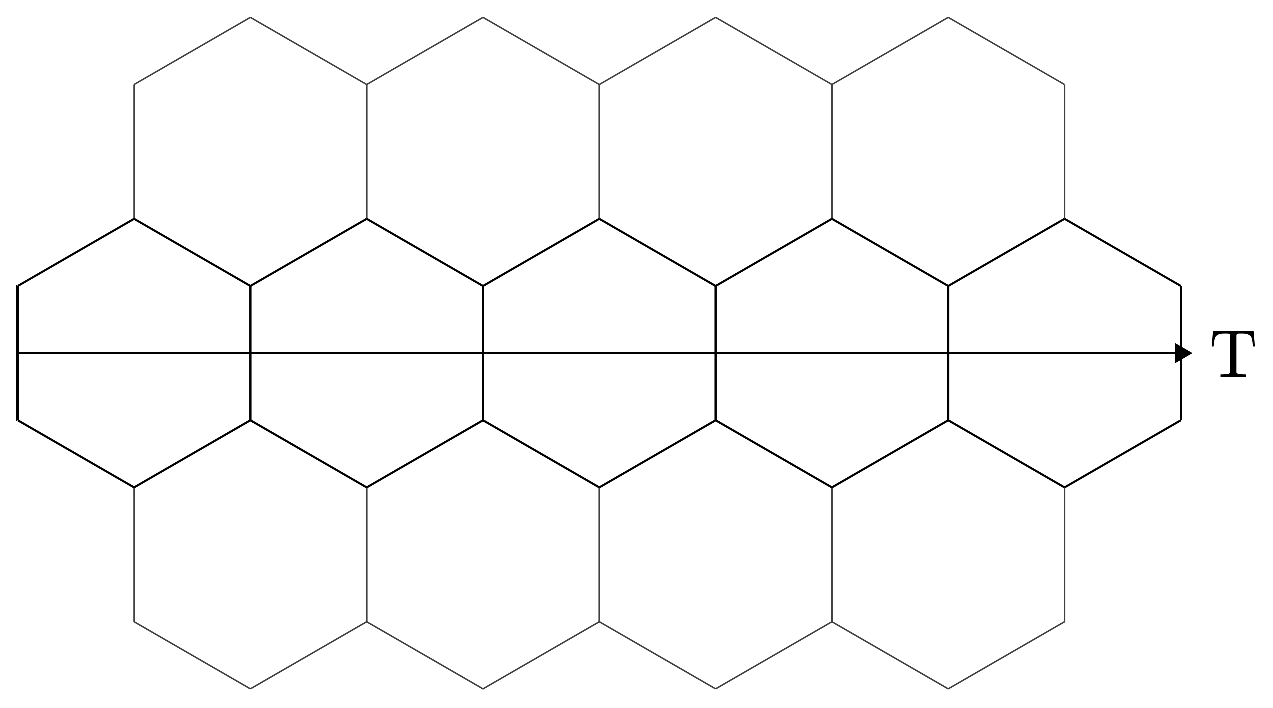
\includegraphics[scale=.25]{./old_fig/Chirality_Armchair.eps}
			\caption{\label{subfig:Armchair}}
		\end{subfigure}%
		~
		\begin{subfigure}[t]{.5\textwidth}
			\centering
			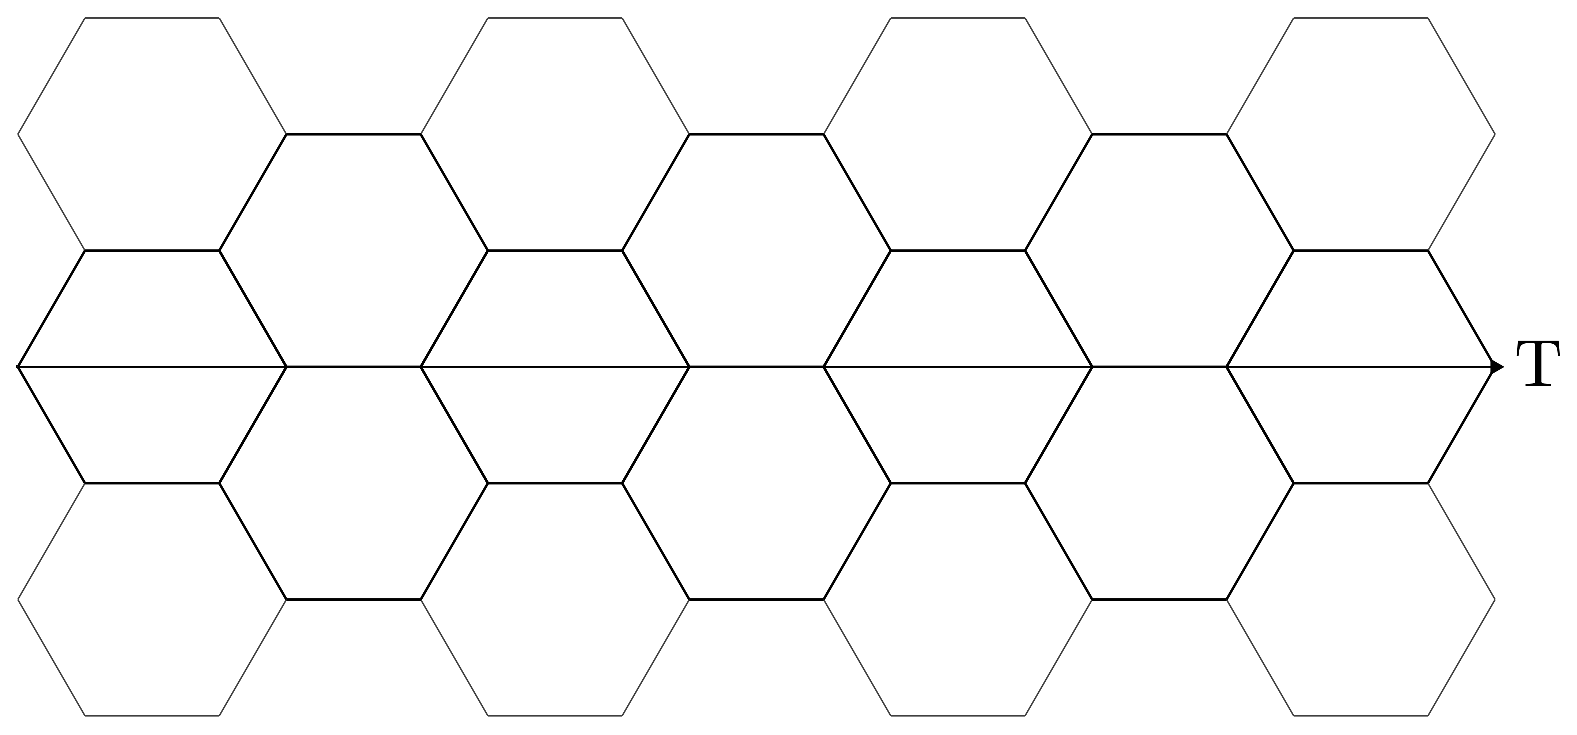
\includegraphics[scale=.25]{./old_fig/Chirality_Zigzag.eps}
			\caption{\label{subfig:Zigzag}}
		\end{subfigure}		
		\caption{Chirality of a CNT can be depicted by how often a hexagonal pattern repeats along a consistent axis. A CNT is (a) armchair if every hexagon is the same, (b) zigzag if the pattern alternates every two hexagons, and chiral otherwise.\label{fig:Chirality}}	
	\end{figure*}
	
\section{Carbon-nanotubes-based materials}

By Carbon-nanotubes-based materials, we mean materials that consist entirely (except for possibly a substrate) of CNTs and no additional materials like polymers.	
The macroscopic properties of CNTs-based materials are dependent on several factors: purity, porosity, and alignment being a few.
A CNT forest, turf, or array is a structure consisting of several CNTs grown from a substrate.
One method for producing CNT forests is chemical vapor deposition.
CVD has been used in nano-electronic fabrication and is not a new technology.
When considered for CNTs it allows for targeted growth on a substrate which is a desirable property for designing and making electronic applications.
CVD is thought to have the best potential for commercial success \cite{Nessim2010}.
A simplified description of CVD is of a furnace that energizes a gas and substrate (usually with some catalyst) to cause a chemical bonding of gas particles with the substrate.
In the case of CNTs the gas consists of hydrocarbons and several different catalysts have been tried and tested.
However, the exact mechanism of CNT growth in a CVD process is complicated by factors such as chemical processes depending on the catalyst, ballistics involving the CNT length \cite{Louchev2003}, and temperature of the CVD.
The quality of the CNT forest can vary greatly and has been considered more of an art than a science \cite{Nessim2010}.  
	
Vertically aligned carbon nanotubes (VACNTs) are used in several different applications.
The electrical and thermal conductivity of CNT materials are highly dependent on the alignment bias of the material.
Likewise adhesive and optical properties of VACNTs are very dynamic and depend on structure, uniformity, purity and other factors.
VACNTs can be used as hydrophobic materials \cite{Lau2003}, dry adhesives \cite{Chen2012}, hologram generators \cite{Montelongo2013}, and nano-workbenches \cite{Gjerde2006}.
VACNTs have an adhesive property and simultaneously have low static friction which plays a critical role in the hydrophobic, and workbench applications.
Xu et al. demonstrate a crowding effect of CNT arrays that allows for control of CNT alignment \cite{Xu2012}.
The structure of a forest can also be used to spin yarns.
A super-aligned array of CNTs can be spun into a yarn of lengths up to centimeters or more \cite{Jiang2002}.
	
A film of CNTs, with no necessary alignment bias or connection to a substrate, is called buckypaper.
Buckypaper is assembled in several ways, including layer-by-layer deposition of functionalized MWCNTs \cite{Lee2008} and ``domino pushing'' of a CNT array.
The relative properties of buckypaper are dependent on the assembly method.
Wang et al. describe the ``domnio pushing'' method as pressing a micropore membrane onto a CNT array.
The membrane is pushed by a cylinder with constant pressure from one end to the other of the CNT array causing individual CNTs to collapse in a ``domino'' fashion.
The CNTs then stick to the membrane and can be peeled off a silicon substrate and then treated and peeled off the membrane \cite{Wang2008}.
A buckypaper assembled with ``domino pushing'' of a highly aligned CNT array will also have an alignment bias, whereas a layer-by-layer deposition will be randomly distributed.

CNTs are often used as a reinforcing agent in composite materials, for example as dispersed CNTs in an epoxy deposit to improve mechanical strength.
A common method of constructing composite materials is through solvents.
In a process involving solvents, CNTs are dispersed with a polymer material and then the solvent is carefully evaporated.
Uniform dispersion of CNTs is a primary concern for mechanical reinforcement, where ideally the stress applied to a material would be augmented by the strength of the reinforcing tubes \cite{Coleman2006}.
There are several composite and reinforcement processes that have been explored and that have varying effectiveness to create an improved composite material.
Spitalsky et al. review several processes and discuss properties of corresponding composites \cite{Spitalsky2010}.

\begin{figure*}[t!]
		\centering
		\begin{subfigure}[t]{.33\textwidth}
			\centering
			
\includegraphics[scale=.25]{./fig/ch1/Nanotube.eps}
			\caption{\label{subfig:Nanotube}}
		\end{subfigure}%
		~
		\begin{subfigure}[t]{.33\textwidth}
			\centering
			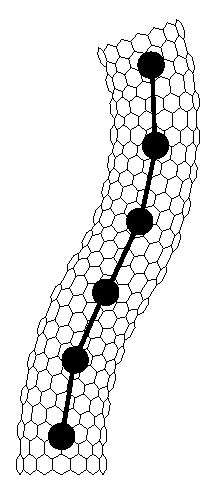
\includegraphics[scale=.25]{./fig/ch1/NanotubeParticle.eps}
			\caption{\label{subfig:NanotubeParticle}}
		\end{subfigure}%
		~		
		\begin{subfigure}[t]{.33\textwidth}
			\centering
			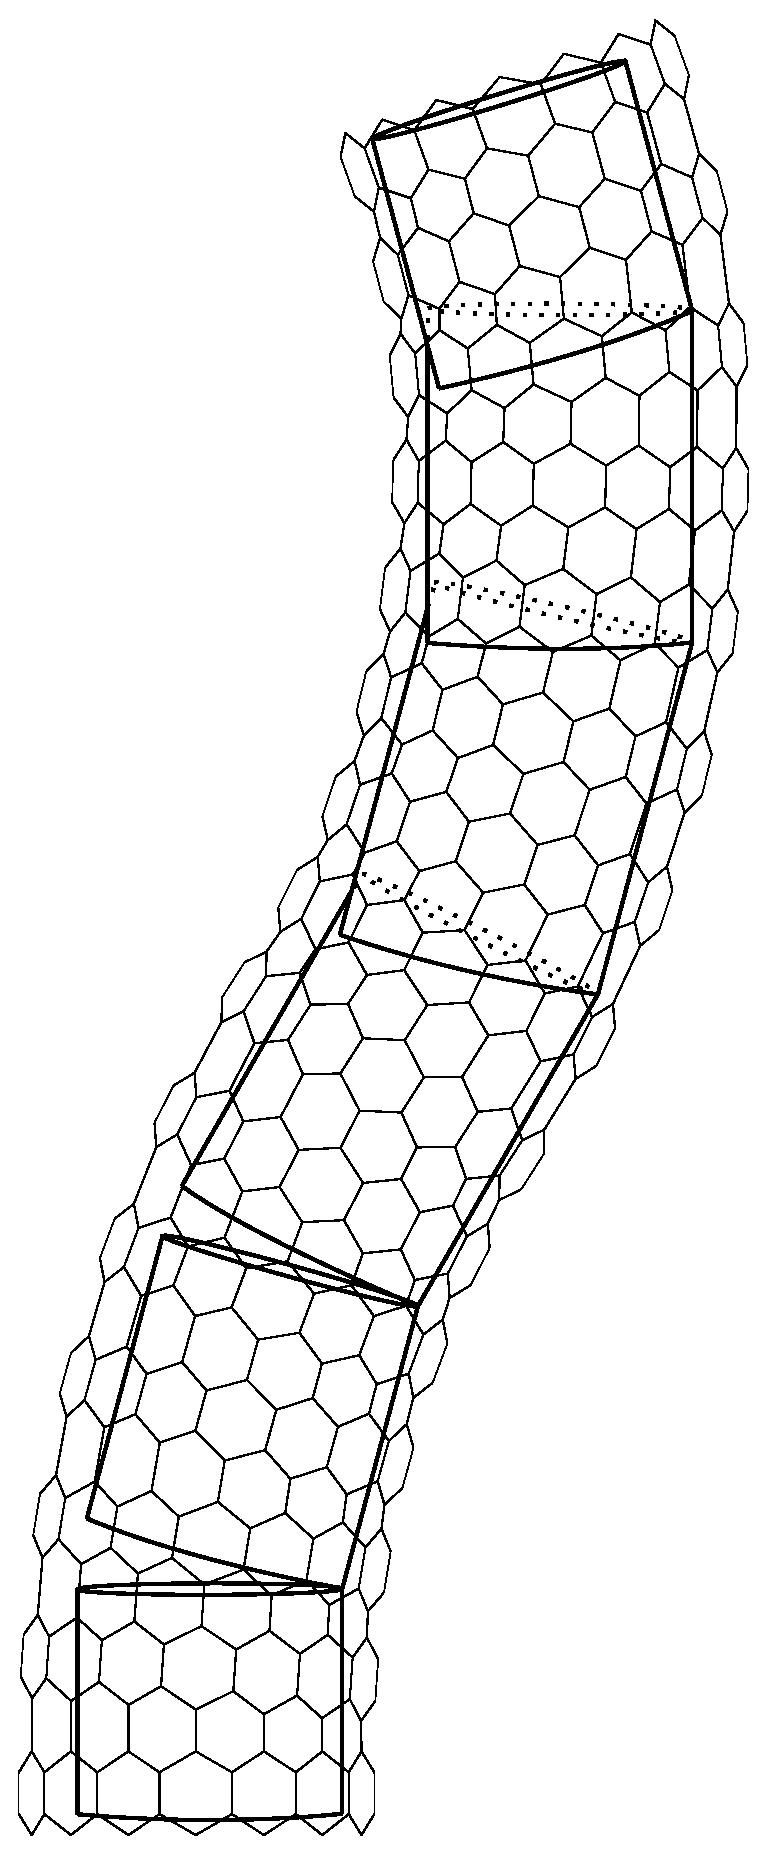
\includegraphics[scale=.25]{./fig/ch1/NanotubeCylinder.eps}
			\caption{\label{subfig:NanotubeCylinder}}
		\end{subfigure}
		\caption{There are several ways to model a CNT with a coarse-grained approach. (a) A CNT under torsional strain can be depicted as (b) a particle bead-spring model of a CNT or (c) a sequence of cylinders model of a CNT. \label{fig:CoarseGrain}}	
	\end{figure*}

\section{Models of buckypaper and fiber materials}

	CNTs in buckypaper can be modeled as individual fibers due to their aspect ratio and flexibility. Indeed, any material consisting of a large volume of CNTs can be thought of as a fiber material. Fiber materials or films are modeled at various length scales. Molecular dynamics takes a small collection of particles and describes their motion with some governing dynamical system for a short period of time. Full atomistic simulations of fiber structures are generally speaking impractical for a large number of atoms or long time scales. For example, investigation of the heat conductance of a single CNT is a practical consideration for molecular dynamics simulations \cite{Maruyama2003}. In order to investigate longer length and time scales coarse-grained approaches are used. The exact time and length scales that are appropriate for different computational techniques are difficult to quantify. With consistently improving hardware and better algorithms and techniques to handle error propagation the line is steadily shifting. However, qualitatively, molecular dynamics approaches will always be focused on a shorter time scale and smaller systems than coarse-grained approaches which in turn are effective at smaller scales than finite element methods \cite{Muller2002}.
	
	Coarse-grained techniques applied to fiber materials model a collection of atoms as a single particle, encapsulating the motion of an entire fiber as a chain of linked particles, instead of a molecular structure of bonded atoms. The focus of coarse-grained simulations is on the mesoscopic scale, somewhere between 1 nanometer and 1 micrometer.  There are many variations to coarse-grained fibers: the fiber can be thought of as a single rod with an attached particle (or a ``lollipop'') \cite{Buehler2006}, a collection of bead-spring links \cite{Li2012} (see Fig.~\ref{subfig:NanotubeParticle}), or a sequence of cylinders \cite{Volkov2008} (see Fig.~\ref{subfig:NanotubeCylinder}).
	
After a model and set of governing equations is developed, the next concern is constructing initial data.
When dealing with a fiber material or mesh with hundreds of fibers, manual generation of initial data is impractical.
Thus appropriate and careful construction of the initial configuration is a concern.
Preventing fibers from penetrating each other and obtaining a desired volume fraction are two of the issues involved in constructing self-consistent initial data.
Dalmas et al. modeled fibers as several splines \cite{Dalmas2006}, however there was no inner volume to each fiber due to an effective zero radius of the fibers which made it difficult to construct a mesh of a desired volume fraction.
Altendorf and Jeulin address this issue with random walks of spheres that can shrink to ``squeeze'' through holes allowing for low porosity \cite{Altendorf2011}.
Cranford et al. construct an array of fibers independently of the mesh and then sediment each array onto a surface \cite{Cranford2010}.

\section{Models of fiber adhesion}

Van der Waals interaction is a combination of several interatomic forces (both repulsive and attractive).
Van der Waals interaction has been considered as a predominant force in adhesive materials (e.g. dry adhesion of Gecko setae \cite{Autumn2002}), and has been used to investigate properties of mesoscopic fibers (e.g. spider silk fibrils \cite{Cranford2013}).
The models we consider here are those that consider van der Waals interaction as a critical mechanism for adhesion of a fiber or fiber material.
A model of fiber adhesion incorporates fibers and possibly other structures like substrates with some adhesive force.
Although fiber only adhesion can and has been considered \cite{Li2011}, we focus on adhesion involving substrates. 
	
	Fu and Zhang utilized an exact continuum model to investigate peeling of a fiber off a substrate \cite{fu2011}. Majidi introduced a continuum model for fiber adhesion with an upper substrate, in particular focusing on the adhered length of a fiber as a function of the applied normal and shear force \cite{Majidi2009}. Majidi's model was later expanded by He et al. to include a coupling effect between shear and normal force \cite{He2012}, and then later to include an axial strain \cite{He2013}. 
	
	To model several interacting fibers, finite element methods have been used \cite{Radhakrishnan2013}. Hu et al. take a multiscale approach adapting coarse-grained molecular dynamics and finite element method to model an array of fibers between two substrates \cite{Hu2010}. Yang et al. investigate a similar problem with only coarse-grained fibers \cite{Yang2012}.
	
	Models of fibers with an adhesive mechanism follow several patterns in the governing energies or forces. Both Hu et al., and Yang et al. include at least a bending energy, axial energy, and short-range potential. Yang et al. stochastically add springs between neighboring fibers to reinforce the several vertically aligned fibers close to the bottom substrate. If there is an axial energy between particles in a coarse-grained fiber it is usually treated as an extensible spring, however inextensible equivalents also exist. The bending of a fiber is usually determined by the interior angle of contiguous particles along the fiber. Finally, the short-range potential models the van der Waals interaction inter-fiber or between fiber and potentially other objects like substrates. 

	We take a similar approach using a simple coarse-grained model with an axial, bending, and short-range weak interaction energies. We also include two substrates, one of which can be rigidly translated by an applied load. The vdW interaction between the fiber and the substrates is explored as a type of adhesion.
	
\section{Summary}

We consider a system consisting of one or more fibers constrained between two parallel substrates where one substrate is stationary, while the other substrate can move. 
The fibers are assumed to be physically attached to the stationary substrate. 
They can be stretched or bent and are subject to non-local self-interactions as well as van der Waals interactions with other fibers and both substrates. 

In Chapter 2, we formulate a coarse-grained model of the fibers/substrates system in which the fibers are replaced by chains of discrete particles connected by extensional and torsional springs and implement this model numerically. 
We assume that dynamics of the system is dominated by dissipative effects and thus can be described in terms of a gradient flow. 

In Chapters 3 and 4, we perform a number of numerical experiments to study the adhesive properties of the fibers. 
First, in Section 3.1, we discard the movable substrate and consider a fiber initially attached orthogonally to the stationary substrate. 
We then determine an equilibrium configuration that results from relaxing the fiber over time. 
We observe that the fiber can either remain free-stranding or adhere to the substrate, e.g., if the torsional springs are sufficiently weak. 
Note that, as in all of our simulations, the equilibrium configuration corresponds to a local minimizer of the energy.

In the next set of experiments in Section 3.2, we reintroduce into the system the rigid movable substrate. 
This (top) substrate can undergo translational motion while remaining parallel to the stationary (bottom) substrate to which the fiber is attached. 
The top substrate is assumed to interact with the fiber via van der Waals forces. Loads of various magnitudes are applied at different angles to the top substrate causing the fiber to deform and adhere to one or both substrates. 
We analyze the set of resulting equilibrium configurations and discuss the dependence of these configurations on material parameters of the system.

The compression experiment is followed by the study of the fiber detachment in Section 3.3, where the sign of the load acting on the top substrate is reversed. 
We investigate dynamics of detachment and identify possible detachment mechanisms. 
Finally, in Chapter~\ref{chap:four}, we present some preliminary results for a two substrate system with multiple fibers.
\chapter{Model} \label{chap:two}

% Parameter Table
\begin{table}
	\rowcolors{1}{}{lightgray}
	\centering
	\caption{Model parameters. \label{table:parameters}}
	\begin{tabular}{c p{.25in} p{4.5in}}
		$m$ & & Number of fibers \\
		$n_j$ & & Number of particles on fiber $j$, $1 \leq j \leq m$ \\
		$n_+$ & & Number of particles on the top substrate \\
		$n_-$ & & Number of particles on the bottom substrate \\
		$\delta_j$ & & Attachment point for fiber $j$ on bottom substrate, $1 \leq j \leq m$ \\
		$\ell$ & & Equilibrium distance for extensible springs \\
		$\ell_+$ & & Spacing between particles on the top substrate \\
		$\ell_-$ & & Spacing between particles on the bottom substrate \\
		$\beta$ & & Strength of torsional springs \\
		$\gamma$ & & Spring constant for extensible springs \\
		$\varepsilon$ & & Strength of vdW force between particles of fibers \\
		$\varepsilon_+$ & & Strength of vdW force between a particle on a fiber and a particle on the top substrate \\
		$\varepsilon_-$ & & Strength of vdW force between a particle on a fiber and a particle on the bottom substrate \\
		$\sigma$ & & Equilibrium distance between two particles for vdW \\
		$(\mu,\lambda)$ & & Load applied to the moving substrate \\
		$(x^{(+)}_0,y^{(+)}_0)$ & & Initial position for first particle on the top substrate \\
		$(x^{(-)}_0,y^{(-)}_0)$ & & Initial position for first particle on the bottom substrate
	\end{tabular}
\end{table}
	
	\begin{figure}
		\begin{center}
			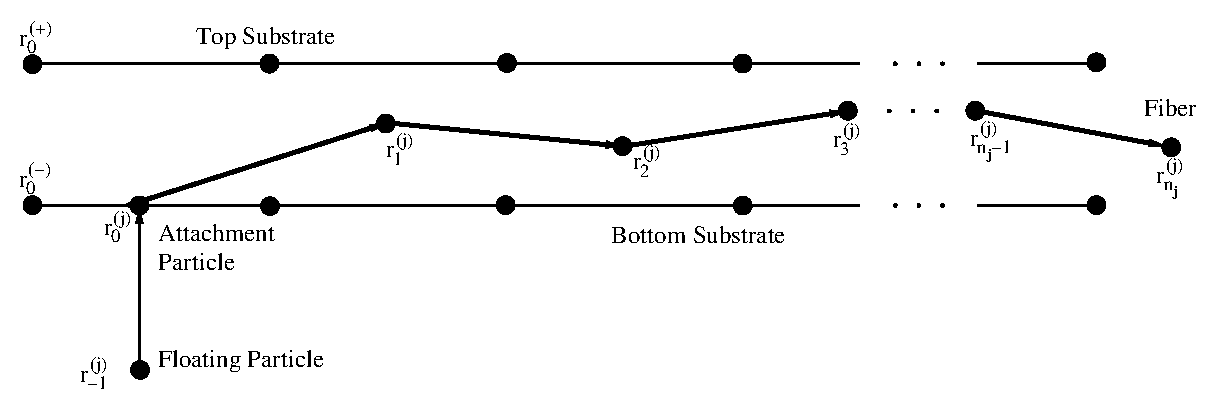
\includegraphics[scale=.75]{./old_fig/Geometry.eps}
		\end{center}		
		\caption{Geometry of a fiber pinned between the top and bottom substrates.
		\label{fig:Geometry}}
	\end{figure}		
	
\section{Geometry}

	We consider a collection of particles linked into a chain that we call a fiber. Each fiber is connected to a stationary horizontal (bottom) substrate at some fixed position. There are two artificial particles associated with each fiber, one being the attachment point with the substrate and an additional particle placed at any point on a half circle below the stationary substrate of radius one. We will call the attachment point the attachment particle, and the other particle below it the floating particle (see Fig.~\ref{fig:Geometry}).
	
We denote the position vector of the $i$th particle on the $j$th fiber by
\begin{equation}
	\textbf{r}_i^{(j)} = (x_i^{(j)},y_i^{(j)})
\end{equation}
where $1 \leq j \leq m$ and $1 \leq i \leq n_j$. We also define the following vectors,

\begin{equation}
	\Delta \textbf{r}_i^{(j)} = \textbf{r}_i^{(j)} - \textbf{r}_{i-1}^{(j)}.
\end{equation}
The two artificial particles are denoted as follows,
\begin{equation}
	\textbf{r}_0^{(j)} = (x_0^{(j)},y_0^{(j)}) = (\delta_j,0)
\end{equation}
for the attachment particle and
\begin{equation}
	\textbf{r}_{-1}^{(j)} = (x_{-1}^{(j)},y_{-1}^{(j)}).
\end{equation}
for the floating particle.

	In any given configuration there could be several fibers, each consisting of a contiguous chain of linked particles. Each particle can be thought of as a discretization of a neighborhood of bonded carbon atoms. Indeed, a chain of particles is intended to describe a CNT via a coarse-grained approach. This approach is sufficiently generic to describe other fiber structures.
	
	In addition to the $m$ fibers in the model are two horizontal substrates, both a top and bottom one. The bottom substrate as described before is attached to every fiber at the attachment particle. We define two sets position vectors,
\begin{eqnarray}
	\textbf{r}_0^{(+)} = (x_0^{(+)},y_0^{(+)}) \\
	\textbf{r}_i^{(+)} = (x_0^{(+)} + i\ell^+,y_0^{(+)})
\end{eqnarray}
for the top substrate and,
\begin{eqnarray}
	\textbf{r}_0^{(-)} = (x_0^{(-)},y_0^{(-)}) \\
	\textbf{r}_i^{(+)} = (x_0^{(+)} + i\ell^-,y_0^{(+)})
\end{eqnarray} 
for the bottom substrate. Both substrates have one predetermined particle, the $0th$ particle. The top substrate is allowed to move under a translational load but the bottom substrate is stationary (see Fig.~\ref{fig:Geometry}).

\section{Energy}

	An isolated fiber is in equilibrium when all particles on a chain are collinear and each particle is a fixed distance $\ell$ away from its neighbors. In order to achieve this equilibria configuration we incorporate two types of springs into the model: an extensible spring and a torsional spring.

\subsection{Extensible spring}

	The extensible spring is described by the standard Hooke's law and is meant to keep any two adjacent particles on a fiber a fixed distance $\ell$ apart. This can also be thought of as maintaining a length of $\ell$ for all links between particles. The energy for all springs is,
\begin{equation}
	E_e = \gamma \sum_{j=1}^m \sum_{i=1}^{n_j} \left[ \left( \|\Delta \textbf{r}_i^{(j)} \| - \ell \right)^2 \right].
\end{equation}
Note that, with our notation for a given fiber $j$ ,the sum starts with the first particle and the attachment particle of that fiber. The sum continues until the final particle on the fiber; it only has one adjacent neighbor.

	\begin{figure}
		\begin{center}
			
\includegraphics[scale=1]{./old_fig/BendingEnergy.eps}
		\end{center}		
		\caption{Two vectors $\textbf{a}$ and $\textbf{b}$, representing links between three particles and a corresponding angle measured against the positive $x$-axis centered at each tail point. The bending energy will be minimized when the difference in angle is zero, or the particles are collinear.
		\label{fig:BendingEnergy}}
	\end{figure}	

\subsection{Torsional spring}

	For a every fiber we want the energy to be minimized when the particles are collinear. To accomplish this we introduce the energy penalty for bending when the angle between adjacent links is not zero (see Fig.~\ref{fig:BendingEnergy}). A quadratic energy is not sufficient here because we expect that the energy should blow up when the links point in opposite directions. Therefore, we set 
\begin{equation}
	e_b = 2 \tan^2 \left( \frac{\Delta \theta}{2} \right),
\end{equation}
where $e_b$ is the energy of one junction between two links since the geometry is described in terms of particles and, not angles, we use double angle identities the definition of dot product to obtain the following expression for total bending energy for every fiber,
\begin{equation}
	E_b = 2\beta \sum_{j=1}^m \sum_{i=1}^{n_j} \left[ \frac{\|\Delta \textbf{r}_i^{(j)} \| \|\Delta \textbf{r}_{i-1}^{(j)} \| - \Delta \textbf{r}_i^{(j)} \cdot \Delta \textbf{r}_{i-1}^{(j)}}{\|\Delta \textbf{r}_i^{(j)} \| \|\Delta \textbf{r}_{i-1}^{(j)} \| + \Delta \textbf{r}_i^{(j)} \cdot \Delta \textbf{r}_{i-1}^{(j)}} \right].
\end{equation}

	This energy incorporates every contiguous set of three particles, including the two artificial particles. With the incorporation of the angle between the artificial particles and the first particle, the minimizing angle of the fiber with respect to the substrate can be tuned according to the placement of the floating particle. For example, if the angle between the floating particle and the attachment particle is $\frac{\pi}{2}$, then the entire fiber will want to be upright, if it is $\frac{\pi}{4}$, then the entire fiber will want be slanted at a $45^{\circ}$ angle, etc.

\subsection{van der Waals interactions}	

	\begin{figure*}[t!]
		\centering
		\begin{subfigure}[t]{.5\textwidth}
			\centering
			\includegraphics[scale=.5]{./fig/ch2/lj_e.eps}
			\caption{Lennard-Jones energy, well depth is $\varepsilon$, minimized at $\sigma$. \label{subfig:LJEnergy}}
		\end{subfigure}%
		~
		\begin{subfigure}[t]{.5\textwidth}
			\centering
			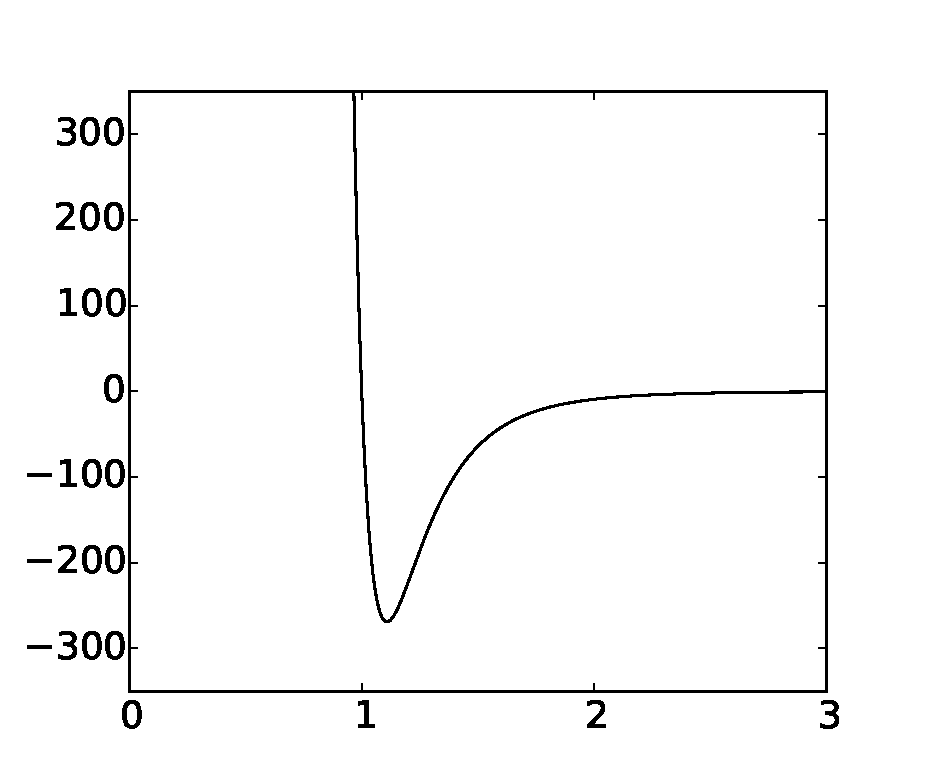
\includegraphics[scale=.5]{./fig/ch2/lj_f.eps}
			\caption{Lennard-Jones force. \label{subfig:LJForce}}
		\end{subfigure}		
		\caption{Lennard-Jones 12-6 potential and force with $\sigma = 1$ and $\varepsilon = 100$.\label{fig:LJ}}	
	\end{figure*}

	At a mesoscopic scale there is typically an interaction between a given particle and every other particle in the system, with $\mathcal{O}(n^2)$ interactions overall Here we use a truncated Lennard-Jones 12-6 potential to represent the van der Waals interactions between each particle in the model. However, because we already have a spring connecting adjacent particles, we don't incorporate an additional interaction between linked particles.
	
The standard Lennard-Jones potential,
\begin{equation}
	U(x) = \varepsilon \left[ \left( \frac{\sigma}{x} \right)^{12} - 2 \left( \frac{\sigma}{x} \right)^6 \right],
\end{equation}

	\begin{figure*}[t!]
		\centering
		\begin{subfigure}[t]{.5\textwidth}
			\centering
			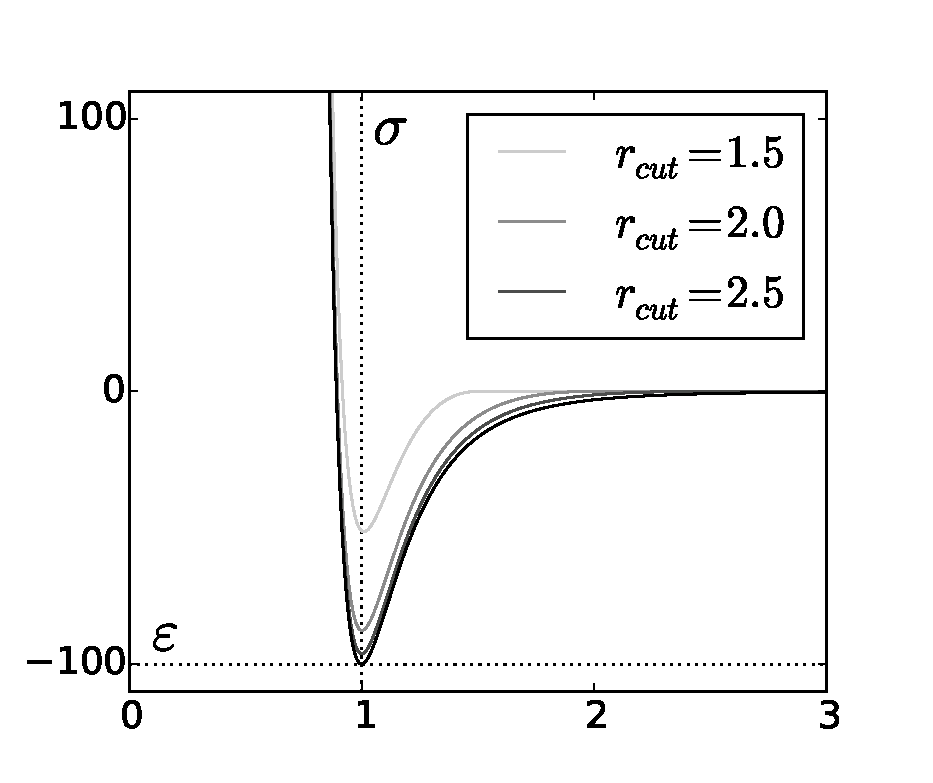
\includegraphics[scale=.5]{./fig/ch2/ljc_e.eps}
			\caption{Truncated Lennard-Jones energy. \label{subfig:LJTEnergy}}
		\end{subfigure}%
		~
		\begin{subfigure}[t]{.5\textwidth}
			\centering
			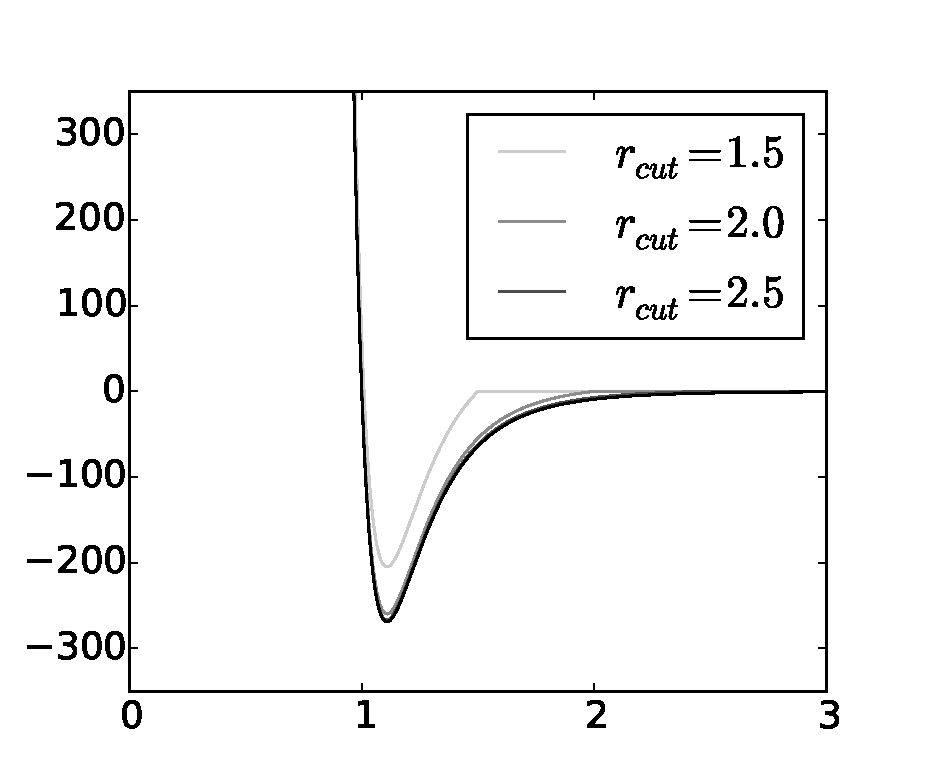
\includegraphics[scale=.5]{./fig/ch2/ljc_f.eps}
			\caption{Truncated Lennard-Jones force. \label{subfig:LJTForce}}
		\end{subfigure}		
		\caption{TODO(new plot with dashed lines and an internal legend) Truncated Lennard-Jones potential with $r_c = 1.5$ in red, $r_c = 2$ in green, $r_c = 3$ in blue, and the Lennard-Jones potential without cut in black.\label{fig:LJT}}	
	\end{figure*}	

\noindent	
asymptotically approaches zero as $x$ approaches infinity. This makes Lennard-Jones a short range potential and, more importantly, makes interactions at long distances negligible. We can then truncate (or cut) the potential at some radius $r_c$. However, this introduces a discontinuity in the potential, so in order to repair both the potential and it's derivative, we use the following modification.
\begin{equation}
	U_c(x) = \left\{ 
		\begin{array}{lr}
			U(x) - U(r_c) - \frac{dU}{dx}\bigg|_{x = r_c}(x - r_c), & x \leq r_c\\
			0, & x > r_c
		\end{array}
		\right. 
\end{equation}

	Clearly the sequence of truncated Lennard-Jones potentials converges to the Lennard-Jones potential as $r_c \to \infty$ and the truncated Lennard-Jones potentials share the same asymptotic behavior (see Fig.~\ref{fig:LJT}). This truncation technique is referred to as a shifted forces, it is commonly used to conserve energy in the potential and avoid potential artifacts with a model. The discontinuous truncation is more commonly used but can cause larger discrepancies in energy particularly with very long simulations. Although this method alters the potential everywhere the accuracy with respect to the true potential is still good, and in specific molecular dynamics simulations it has been observed as better than our alternative \cite{Toxvaerd2011}.
	
	For our model the potential is safer but likely unneeded due to our liberal cutoff selection of $r_c = 8$ in all simulations. However we are searching for equilibrium which can cause very long time intervals over the entire simulation, so to avoid artifacts in the geometry we use this variation of the truncated Lennard-Jones potential.

	In order to represent concisely the set of particles that a given particle is interacting with, we define the set
\begin{equation}
	P(j,i) = \{ (h,k)|j \neq h \vee k \neq i \pm 1, 1 \leq h \leq m, 1 \leq k \leq n_h \},
\end{equation}
which contains every particle that the $i$th particle on the $j$th fiber will be interacting with via the 12-6 potential. We now have the van der Waals energy for all pairs:
\begin{multline}
	E_v = \sum_{j=1}^m \sum_{i=1}^{n_j} \bigg[ \sum_{(h,k) \in P(j,i)} U_c \left( \| \textbf{r}_i^{(j)} - \textbf{r}_k^{(h)} \| \right) \\ + \sum_{k=1}^{n_-} U_c \left( \| \textbf{r}_i^{(j)} - \textbf{r}_k^{(-)} \| \right) + \sum_{k=1}^{n_+} U_c \left( \| \textbf{r}_i^{(j)} - \textbf{r}_k^{(+)} \| \right) \bigg],
\end{multline}
It is not necessarily the case that the interaction strength, $\varepsilon$, is the same for each potential. There are different strengths for fiber to fiber, fiber to top substrate, fiber to bottom substrate interactions respectively.

% van der Waals lower substrate pressure
%\begin{equation}
%	E_p = \sum_{j=1}^m \sum_{i=1}^{n_j} U_p \left( y_i^{(j)} \right)
%\end{equation}

\subsection{Total energy}

To complete the governing equation for the energy we also incorporate a vector load on the top substrate. In particular we apply a translational load to the point $(x_0^{(+)},y_0^{(+)})$. Adding up all contributions gives the total energy, 

% Total energy
\begin{equation}
	E = E_b + E_e + E_v + \lambda x_0^{(+)} - \mu y_0^{(+)}.
\end{equation}

\section{Dynamics}

Using Newton's second law with a damping term we have,

\begin{equation}
	M\frac{d^2\textbf{r}_i^{(j)}}{dt^2} + \frac{d\textbf{r}_i^{(j)}}{dt} = -\nabla_{\textbf{r}_i^{(j)}}E,
\end{equation}

	for some particle, where $M$ is the mass of that particle. We then assume the mass of particles we want to take into consideration is small enough to make the acceleration negligible, which leaves us with,
	
\begin{equation}
	 \frac{d\textbf{r}_i^{(j)}}{dt} = -\nabla_{\textbf{r}_i^{(j)}}E.
\end{equation}

Clearly in solving this ordinary differential equation we are minimizing the total energy of our system. Our first consideration then is to discuss minimizing equilibria of the total energy and second to discuss any dynamical considerations.

TODO(expand)

\section{Implementation}

	The model was first implemented using MATLAB \cite{MATLAB2010}, and then later translated into C using SUNDIALS\cite{sundials}. A Verlet neighbor list is used and dynamically updated at every time step when the sum in the two largest changes in position is greater than the buffer distance in the Verlet list (a static value of 4 in all simulations presented here). A simulation is considered in equilibrium when the max norm of the difference between the latest two solution vectors is less than a prescribed tolerance, and the difference between the latest two top substrate positions is less than the same tolerance. The system is also considered in equilibrium if the velocity of the top substrate is within the same tolerance of it's maximum velocity. Either of these conditions must be satisfied for ten time steps. The equilibrium tolerance is a static value, $10^{-8}$. Matplotlib was also used for several figures presented in this thesis \cite{Hunter2007}.








\chapter{Single fiber simulations}

Although coarse-grained models of a similar nature can and have been fitted to match the properties of a CNT \cite{Cranford2010}, here we focus on exploring the behavior of the model. To that end we are interested in four stages of the model. First, under what circumstances will a fiber not crystallize with the bottom substrate. Second, what configurations or modes of failure are relevant and observable from various loads applied to the fiber by the top substrate. Third, after being equilibrated in an adhered state (that is, the top substrate adhered to the fiber), what kinds of loads are required to detach the top substrate from the fiber and what configurations are observable intermittently. Finally, if the fiber does successfully detach, under what circumstances will it not crystallize with the bottom substrate.

\section{Free standing}

	\begin{figure}
		\begin{center}
			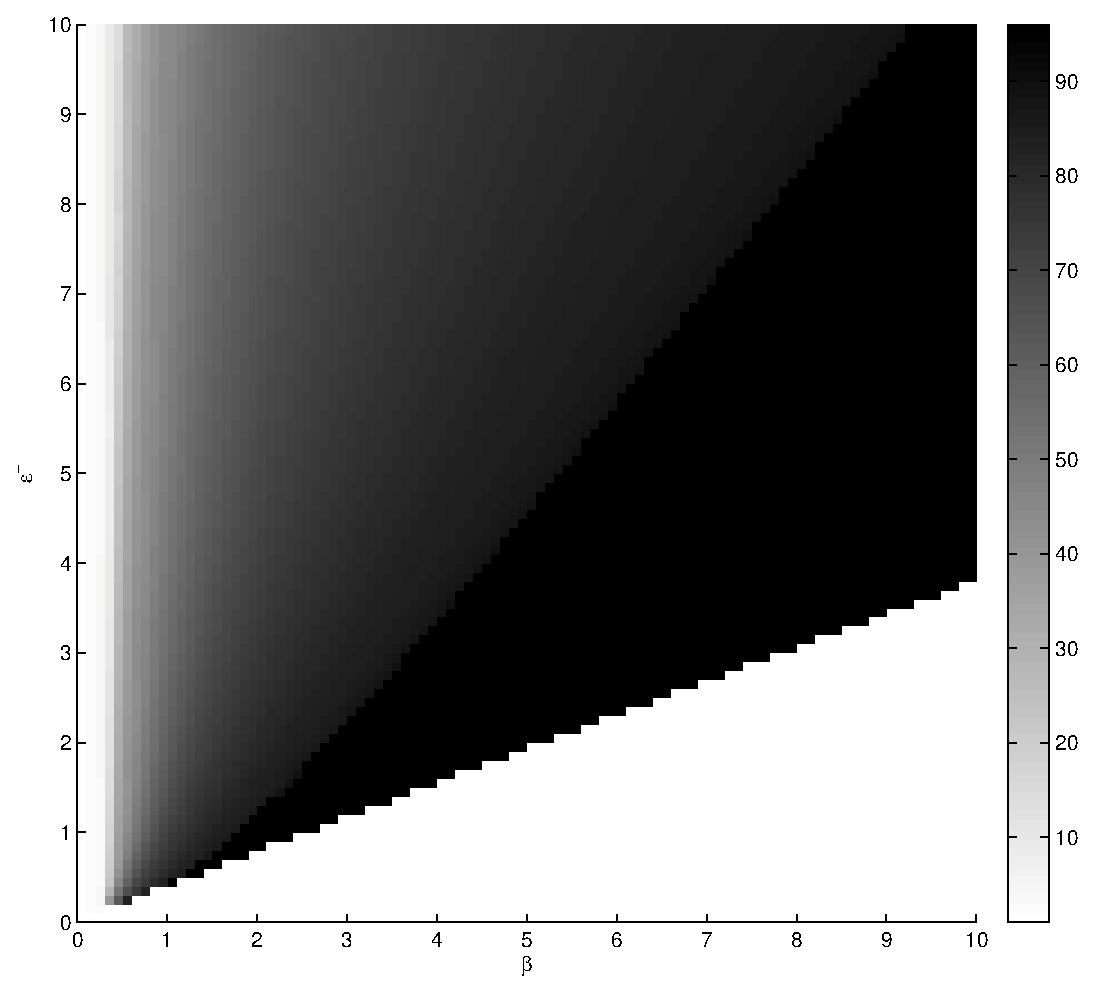
\includegraphics[scale=.5]{./fig/sims/freestanding/fs.eps}
		\end{center}		
		\caption{Phase plot of a fiber's torsional spring strength, $\beta$, against the strength of the bottom substrate's vdW force, $\eps^-$.
		\label{fig:FreeStandingGrid}}
	\end{figure}	

We say a fiber, or part of a fiber, is \textit{crystallized} if the van der Waals energy between a set of particles appears qualitatively to be minimized. If a particle on the fiber is crystallized with two particles on the top substrate we say that it is \textit{adhered} to the top substrate. We define a function to describe how adhered a fiber is to the top substrate in general. Therefore, we define


\begin{eqnarray}
	A(\textbf{a}, \textbf{b}) = \left\{ 
		\begin{array}{ll}
			1, & \|\textbf{a} - \textbf{b}\| \leq 2^{\frac{1}{6}} \sigma + 10^{-6}\\
			0, & \mbox{otherwise}
		\end{array}
		\right.  \\
	A^+ = \sum_{k=1}^{n^+} \sum_{j=1}^{m} \sum_{i=1}^{n} A(\textbf{r}_i^{(j)},\textbf{r}_k^{(+)}) \label{eqn:adhesion:top} \\ 
	A^- = \sum_{k=1}^{n^-} \sum_{j=1}^{m} \sum_{i=1}^{n} A(\textbf{r}_i^{(j)},\textbf{r}_k^{(-)}) \label{eqn:adhesion:bottom}
\end{eqnarray}

If a fiber is not strong enough to prevent crystallization with the bottom substrate without external influence then it is impossible that the fiber will be about to recover from a detachment force. Moreover, the compression with the top substrate will be uninteresting if the fiber is already laying flat in a position the substrate can not effect. Therefore it is pertinent to categorize what parameters cause a fiber to stay upright or at least not crystallize in some capacity. Here we show that $\beta$ and $\eps^-$ play the key role in whether or not the fiber crystallizes (Fig.~\ref{fig:FreeStandingGrid}). The only other parameters that could play a role are: $\sigma$, $\ell$, $\eps$, and $gamma$. With the exception of $\eps$ none of these parameters will have any effect on keeping the fiber standing, but more how the fiber crystallizes or stacks with the bottom substrate. The inner fiber van der Waals interaction strength, $\eps$, is assumed to play a negligible role.

The modes a fiber free from the top substrate are categorizable as collapsed, folded, crystallized, and slanted. These can be immediately seen in figure \ref{fig:FreeStandingGrid}. The white section sufficiently distant from the origin is slanted, the black section above it collapsed, and sufficiently close to the y-axis is crystallized.

	%% Erect Figures
	\begin{figure*}
		\centering
		\begin{subfigure}{.5\textwidth}
			\centering
			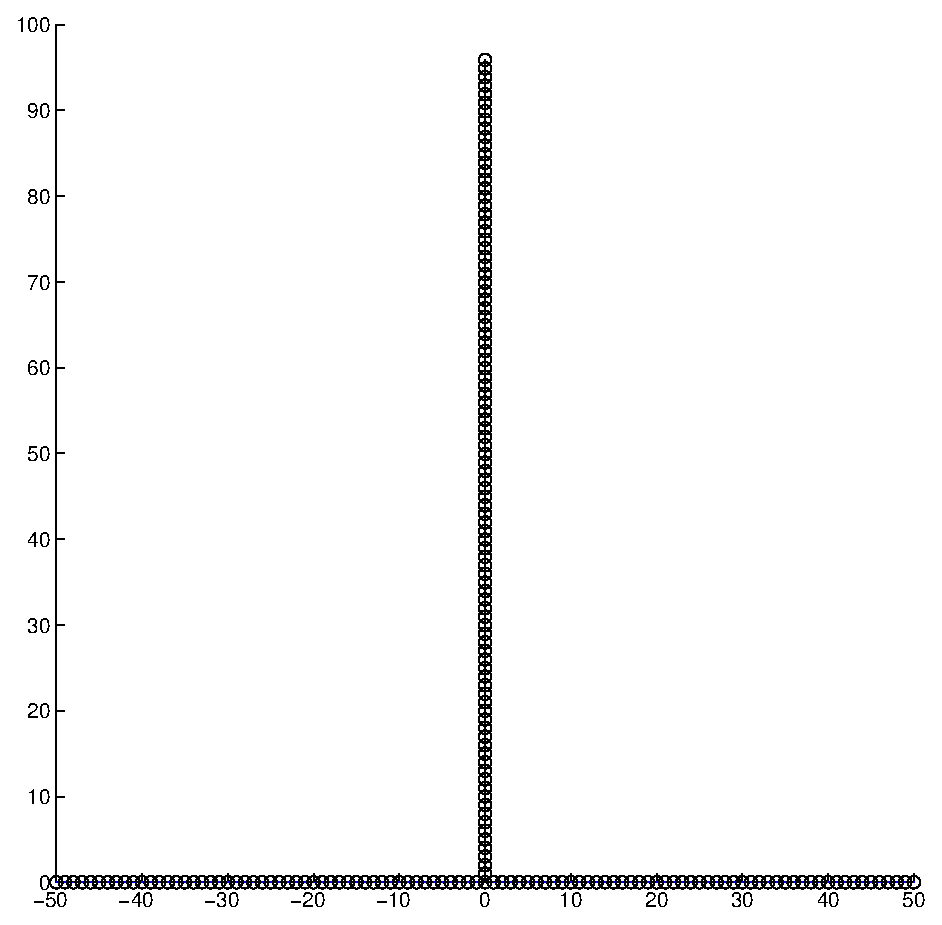
\includegraphics[scale=.4]{./fig/sims/freestanding/erect.eps}
			\caption{TODO \label{subfig:fs_erect}}
		\end{subfigure}%
		~
		\begin{subfigure}{.5\textwidth}
			\centering
			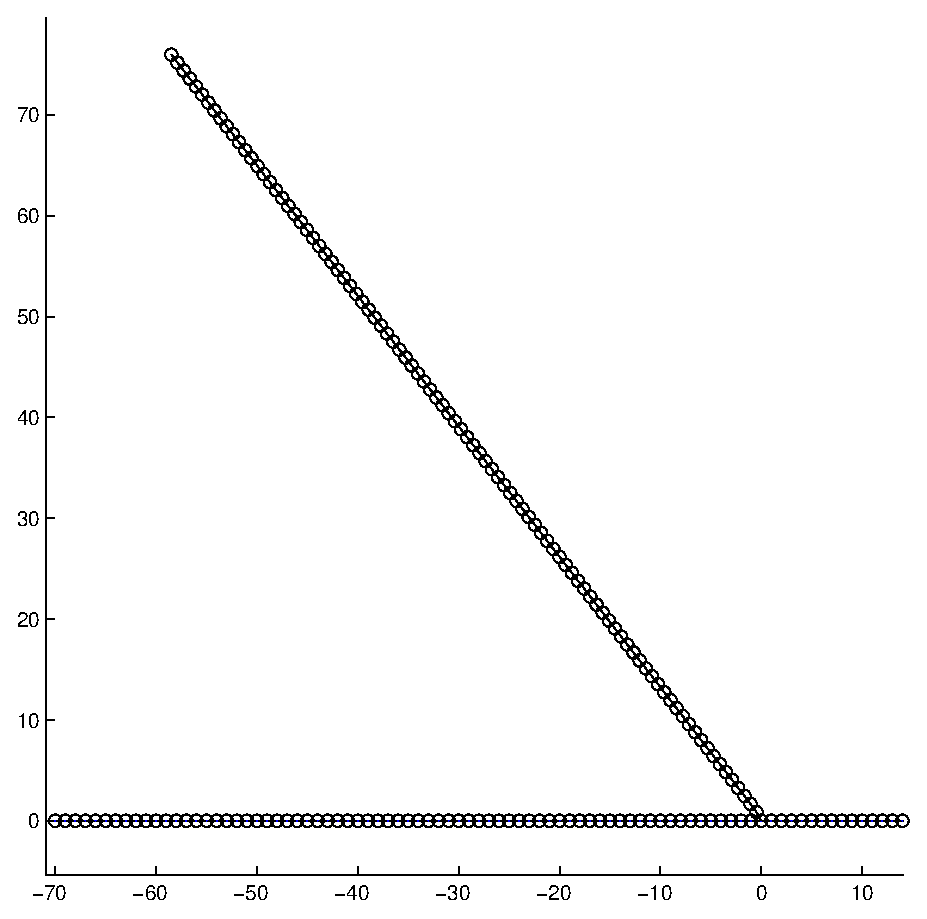
\includegraphics[scale=.4]{./fig/sims/freestanding/erect_leaning.eps}
			\caption{TODO\label{subfig:fs_erectlean}}
		\end{subfigure}
		\caption{TODO\label{fig:fs_erect}}
	\end{figure*}
	
	%% Fallen Figures
	\begin{figure*}
		\centering
		\begin{subfigure}{.5\textwidth}
			\centering
			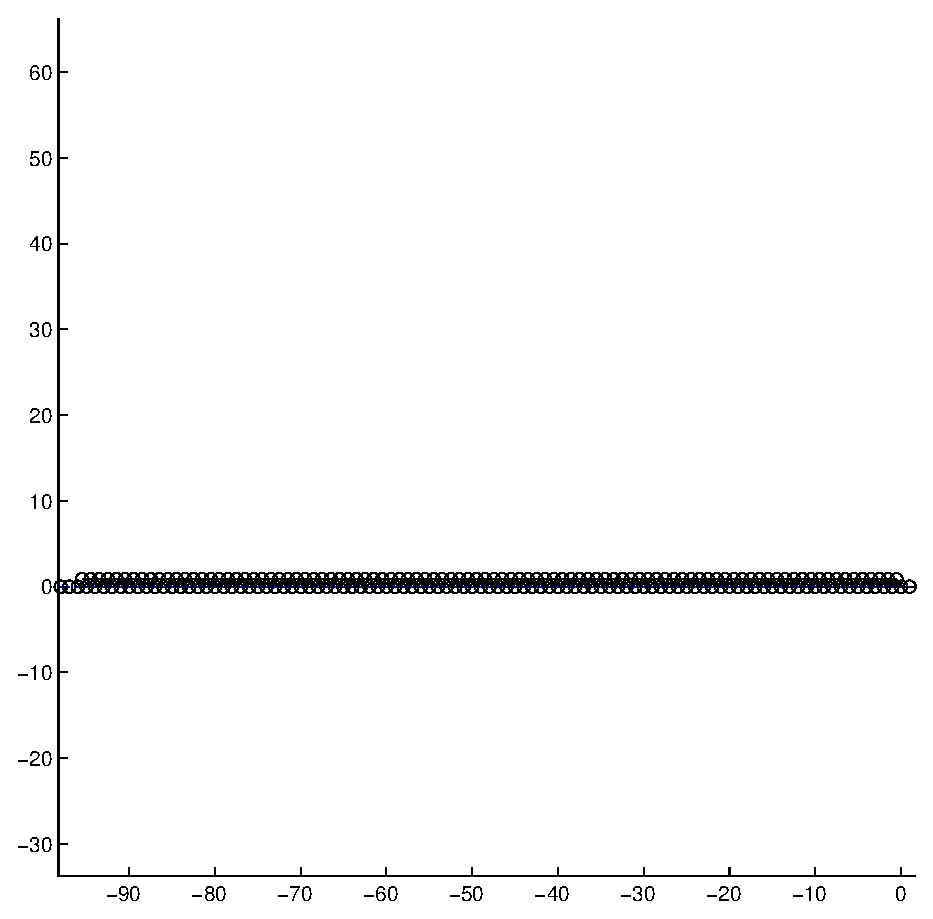
\includegraphics[scale=.4]{./fig/sims/freestanding/completely_down.eps}
			\caption{TODO \label{subfig:fs_down}}
		\end{subfigure}%
		~
		\begin{subfigure}{.5\textwidth}
			\centering
			\includegraphics[scale=.4]{./fig/sims/freestanding/one_fold.eps}
			\caption{TODO \label{subfig:fs_onefold}}
		\end{subfigure}

		\begin{subfigure}{.5\textwidth}
			\centering
			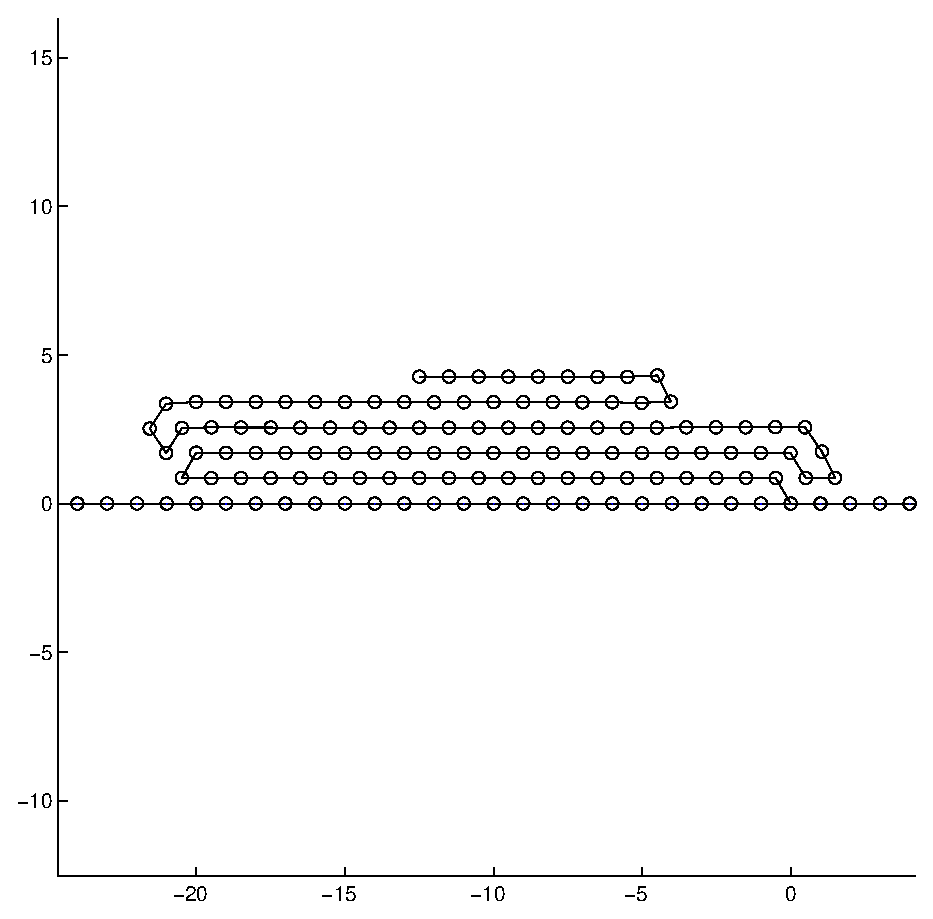
\includegraphics[scale=.4]{./fig/sims/freestanding/many_folds.eps}
			\caption{TODO \label{subfig:fs_manyfold}}
		\end{subfigure}		
		\caption{TODO\label{fig:fs_folds}}	
	\end{figure*}
	
	%% Crystalized Figures
	\begin{figure*}
		\centering
		\begin{subfigure}{.5\textwidth}
			\centering
			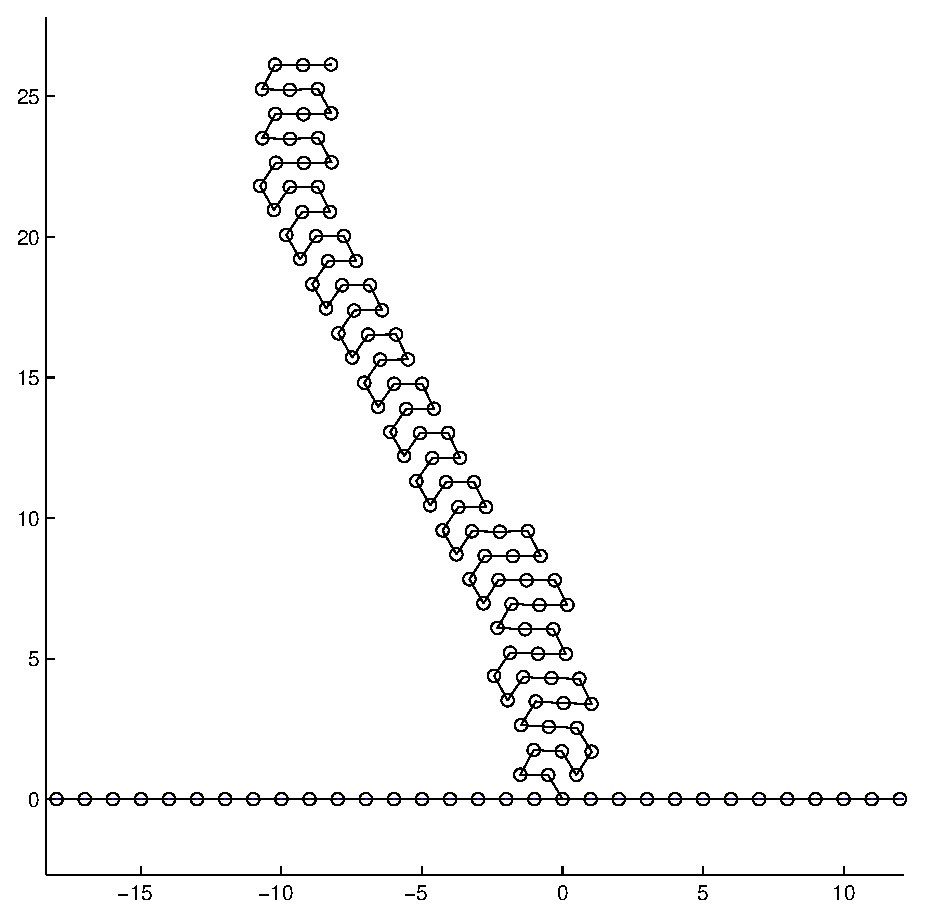
\includegraphics[scale=.4]{./fig/sims/freestanding/crystal1.eps}
			\caption{TODO \label{subfig:fs_crystal1}}
		\end{subfigure}%
		~
		\begin{subfigure}{.5\textwidth}
			\centering
			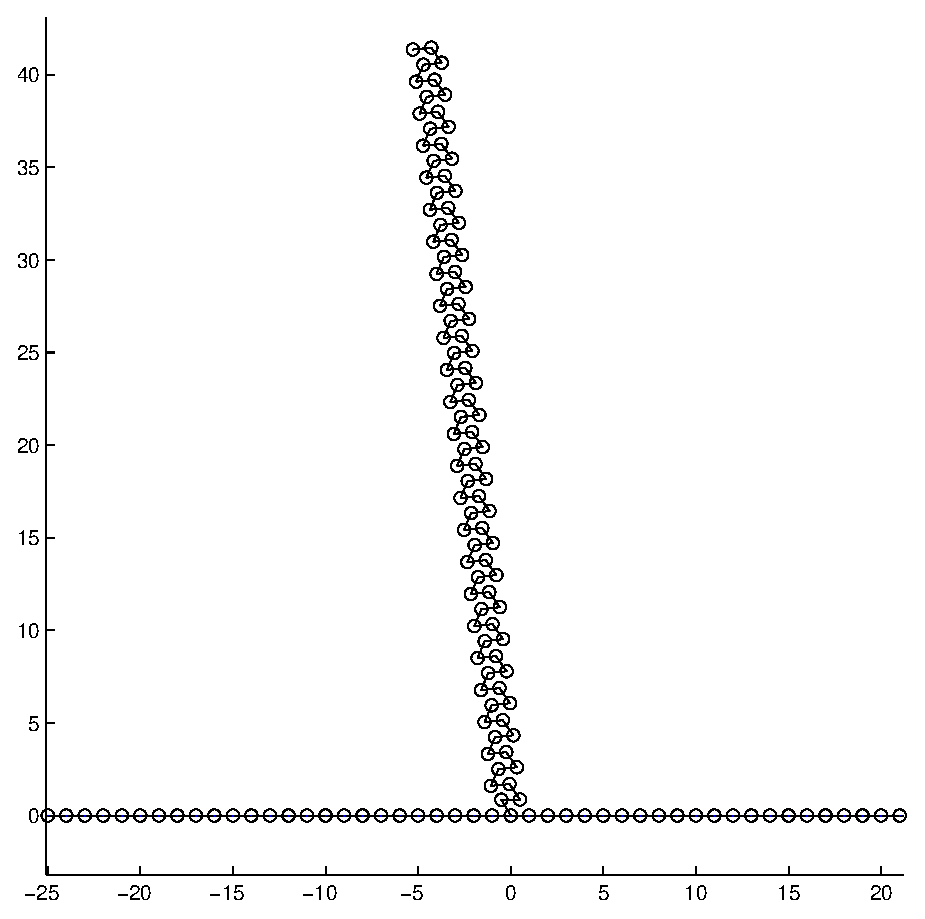
\includegraphics[scale=.4]{./fig/sims/freestanding/crystal2.eps}
			\caption{TODO \label{subfig:fs_crystal2}}
		\end{subfigure}

		\begin{subfigure}{.5\textwidth}
			\centering
			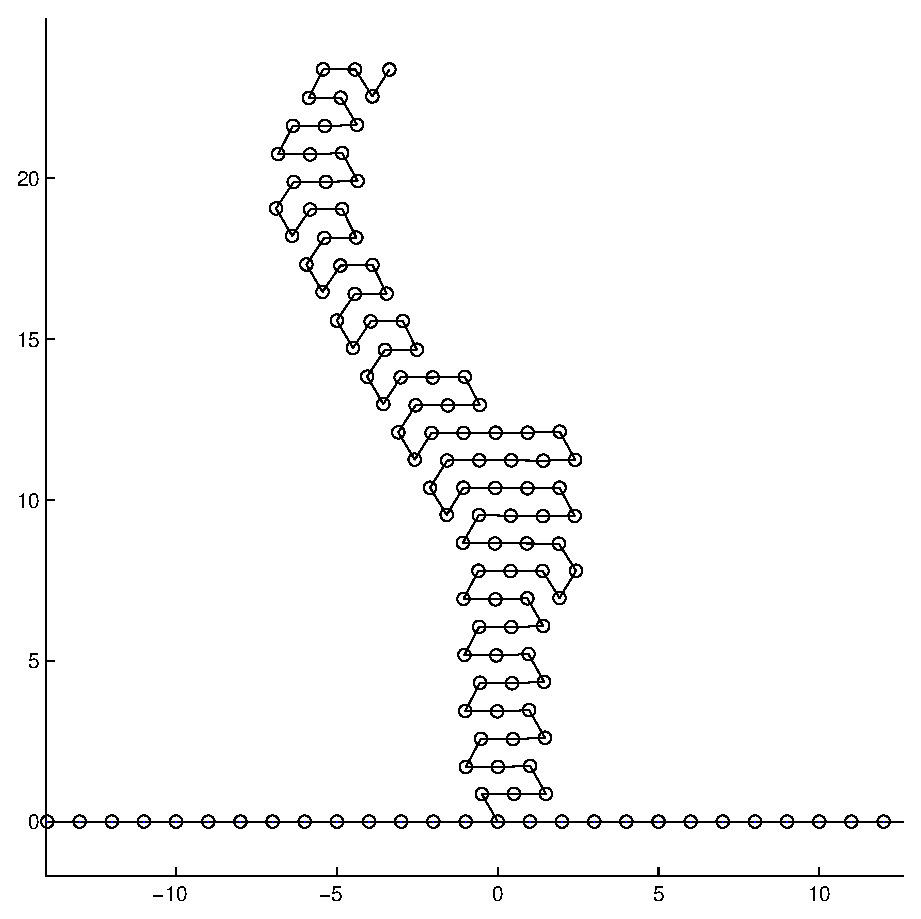
\includegraphics[scale=.4]{./fig/sims/freestanding/crystal3.eps}
			\caption{TODO \label{subfig:fs_crystal3}}
		\end{subfigure}		
		\caption{TODO\label{fig:fs_crystal}}	
	\end{figure*}

Focusing on the slanted mode it is suggested from figure \ref{fig:FreeStandingGrid} that as $\beta$ increases the ability to be slanted does so as well. If we are to look at a fiber in equilibrium near the x-axis we would see figure \ref{subfig:fs_erect} with an indistinguishable slant from being completely up right. As we increase $\eps^-$ from this position the fiber will begin to slant more dramatically. The slant in fiber will be mostly, if not completely, caused by a buckling at the root (see Fig.~\ref{subfig:fs_erectlean}). This can be understood for two reasons. First, the first particle on the fiber that can be bent by van der Waals is also closest to the bottom substrate and thus under it's greatest strain. Second, if the force pulling on the first particle is not strong enough to cause it to crystallize, then surely it will be significantly weaker for the second particle in the chain. This observation implies another important fact, namely, that if the van der Waals interaction can crystallize with the bottom substrate, then the entire fiber will collapse. The immediate change from the slanted mode to the collapsed mode is explained by this importance on the strength of the first torsional spring.
	
The continued increase in $\eps^-$ pushes the mode from slanted to collapsed and near the darkest areas we have a completely collapsed fiber (see Fig.~\ref{subfig:fs_down}). There is another sharp jump as we continue increasing $\eps^-$. The fiber switches from being completely collapsed with the bottom substrate to folding in on itself during the collapsing (see Fig.~\ref{subfig:fs_onefold}). As $\beta$ becomes too weak to maintain a stiffness to the fiber a buckle forms as it collapses. With particles on the fiber collapsing quickly the short-range nature of van der Waals leaves particles just far enough to be left "on top" of previous collapsing particles, only to quickly be taken over by the van der Waals interaction between the bottom substrate and also now the inter-fiber interaction, causing a fold. As we increase $\eps^-$ the number of folds increase as well (see Fig.~\ref{subfig:fs_manyfold}).
	
Moving towards the y-axis we find ourselves encountering a less predictable beast. With $\beta$ very weak there are several crystallization effects that happen to the fiber (see Fig.~\ref{fig:fs_crystal}). In all examples shown the crystallization is primarily inter-fiber. That is, the fiber doesn't seem to collapse, so much as crystallize with itself before it can. (TODO need precise values for these examples, and really all the above figures)

\section{Compression}

	\begin{table}
		\rowcolors{1}{}{lightgray}
		\centering
		\caption{Reference parameters for compression. \label{table:compression_reference}}
		\begin{tabular}{lcrclcr}
			$m$ & = & 1 & \hspace{1in} & $\ell_-$ & = & 1 \\
			$n$ & = & 96 & & $\ell_+$ & = & 1 \\
			$n_+$ & = & 400 & & $\ell$ & = & 1 \\
			$n_-$ & = & 200 & & $\gamma$ & = & 100 \\
			$x^{(-)}$ & = & -100 & & $\beta$ & = & 10 \\
			$y^{(-)}$ & = & 0 & & $\eps^-$ & = & 1 \\
			$x^{(+)}$ & = & -200 & & $\eps^+$ & = & 1 \\
			$y^{(+)}$ & = & 110 & & $\eps$ & = & 1 \\
			$\delta$ & = & 0 & & $\sigma$ & = & 1
		\end{tabular}
	\end{table}

	\begin{figure}[t!]
		\begin{center}
			\includegraphics[scale=1]{./fig/temp.eps}
			%\includegraphics[scale=.5]{./fig/sims/push/p.eps}
		\end{center}		
		\caption{ TODO
		\label{fig:PushGrid:vanilla}}
	\end{figure}	
	
	\begin{figure*}
		\centering
		\begin{subfigure}{.5\textwidth}
			\centering
			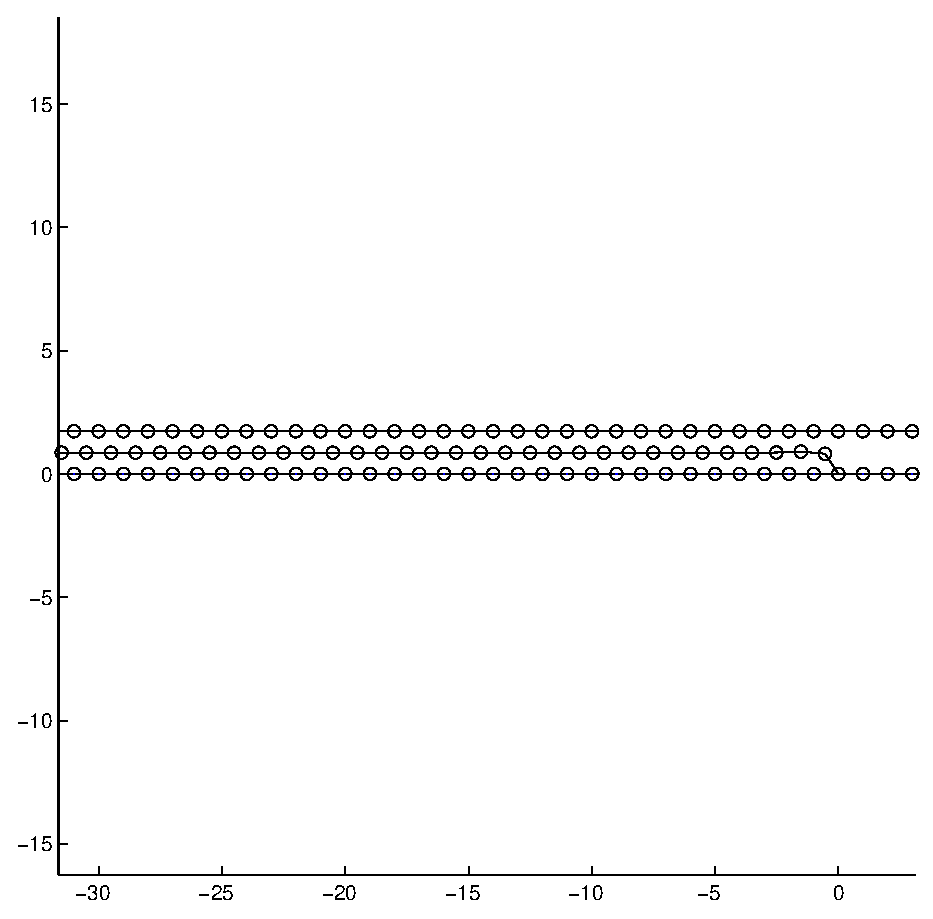
\includegraphics[scale=.4]{./fig/sims/push/squished.eps}
			\caption{TODO\label{subfig:push_squished}}
		\end{subfigure}%
		~
		\begin{subfigure}{.5\textwidth}
			\centering
			\includegraphics[scale=.4]{./fig/sims/push/one_fold.eps}
			\caption{TODO \label{subfig:push_one_fold}}
		\end{subfigure}

		\begin{subfigure}{.5\textwidth}
			\centering
			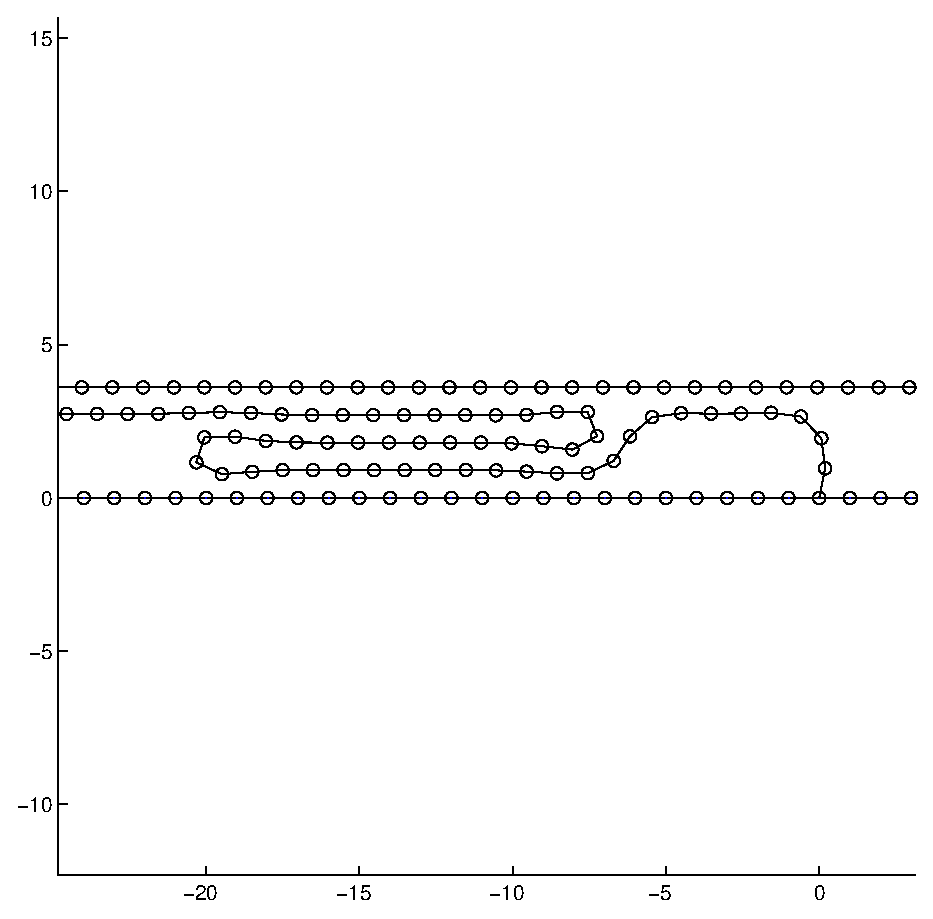
\includegraphics[scale=.4]{./fig/sims/push/two_folds.eps}
			\caption{TODO\label{subfig:push_two_folds}}
		\end{subfigure}
		\caption{TODO\label{fig:push_fold}}
	\end{figure*}

	\begin{figure*}
		\centering
		\begin{subfigure}{.5\textwidth}
			\centering
			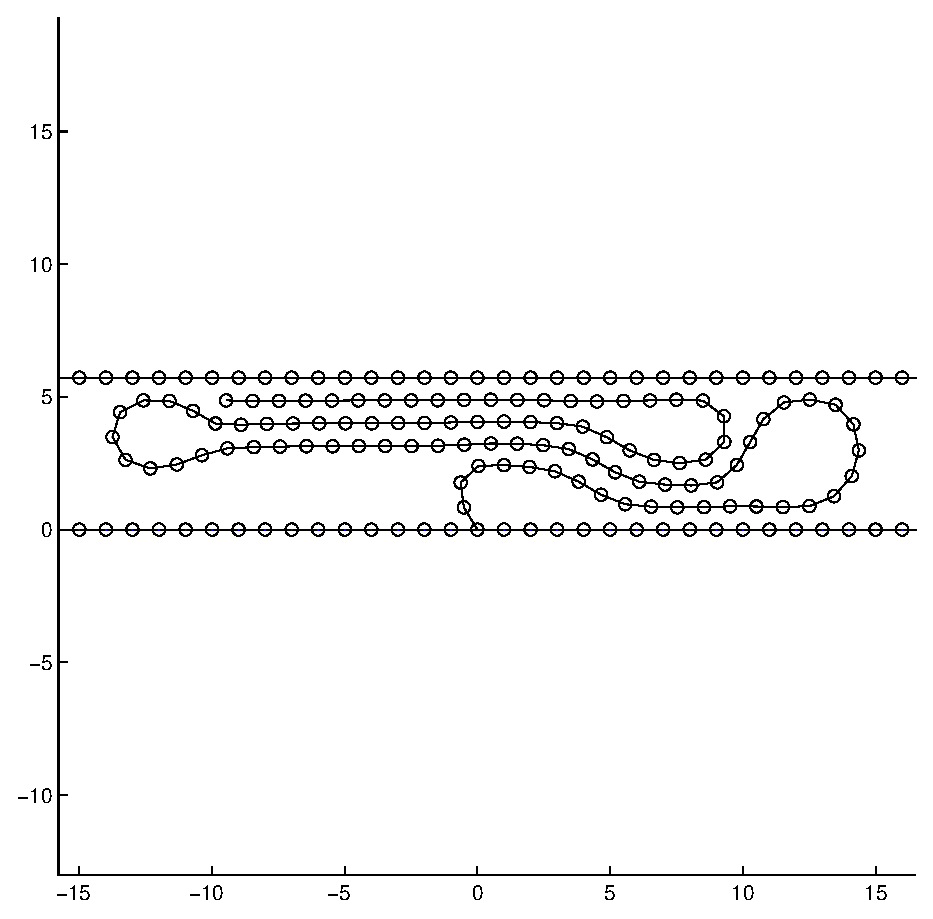
\includegraphics[scale=.4]{./fig/sims/push/curled1.eps}
			\caption{TODO \label{subfig:push_curled1}}
		\end{subfigure}%
		~
		\begin{subfigure}{.5\textwidth}
			\centering
			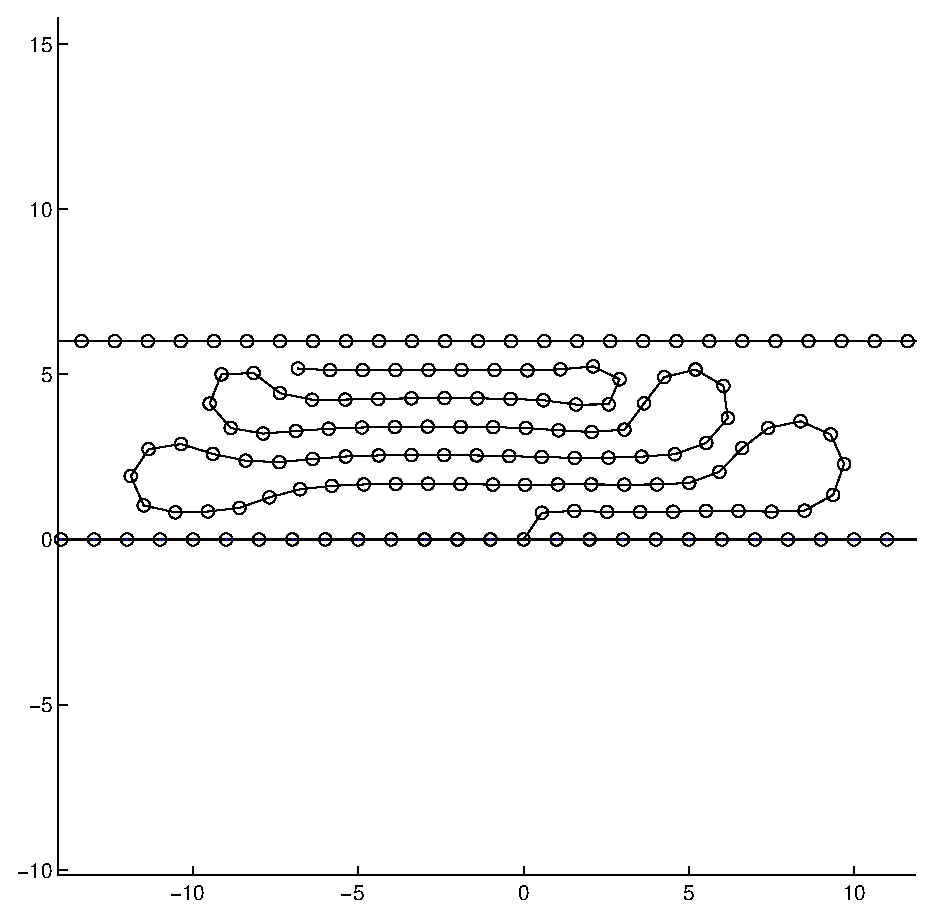
\includegraphics[scale=.4]{./fig/sims/push/curled2.eps}
			\caption{TODO\label{subfig:push_curled2}}
		\end{subfigure}
		\caption{TODO\label{fig:push_curled}}
	\end{figure*}

The compression of a fiber by a load is likely to cause it to buckle. We investigate here under what parameters it will buckle and how it buckles. In all simulations the fiber starts standing vertically and in equilibrium (under the equilibrium criteria described in Chapter~\ref{chap:two}). The top substrate starts a distance far enough away from the fiber so that the cut off Lennard-Jones prevents it from interacting. The experiment begins with a load on the top substrate moving it towards the fiber and bottom substrate. In every configuration we have found under this experiment there is some degree of crystallization between particles on the fiber and particles on the top substrate. Therefore we use the adhesion metric (see Equation~\ref{eqn:adhesion:top}) to differentiate between different buckling configurations. All experiments are done against a set of reference parameters (see Table~\ref{table:compression_reference}). These values have minor significance; a value is chosen to be one unless there is otherwise reason not to. The starting position and particle count for substrates are chosen so that if a fiber were to collapse under any extreme it doesn't run out of particles on either substrate to interact with. This is a guarantee for the bottom substrate based on the chosen values but the top substrate can still ``miss'' the fiber since it has only finitely many particles. Both $\gamma$ and $\beta$ were selected to keep the fiber vertical when not under load, and $\delta$ was chosen to be zero for aesthetics.

\subsection{Observations of Reference Parameters}

Given the reference parameters in Table~\ref{table:compression_reference} we have a diagram, Figure~\ref{fig:PushGrid:vanilla}, demonstrating different buckling configurations after the system is in equilibrium. There is one configuration we focus on in detachment specifically that we can observe. The fiber is said to be \textit{flattened} between the top and bottom substrate when it has completely crystallized with the top substrate and no torsional spring, with the exception of the root, is bent (see Figure~\ref{subfig:push_squished}). This is the starting configuration, after relaxation, for the detachment experiment. Figure~\ref{fig:PushGrid:vanilla} also demonstrates a relationship between an angled load and a flattened configuration. The fiber is said to have a \textit{fold} when one or more particle of the fiber has crystallized with other particles on the fiber. When the load is near $\frac{\pi}{2}$ we start to see folds (see Figure~\ref{fig:push_fold}). When the substrate is even closer, or directly down, the fiber starts to buckle immediately causing more folds in configurations as shown in Figure~\ref{fig:push_curled}.

Flattened fibers occur under these parameters when the angle of the load is sufficiently away from $\frac{\pi}{2}$. An explanation for this behavior is that as the fiber buckles it crystallizes with the top substrate and is sheared by the horizontal component of the load to be ``zipped'' to the top substrate. A fiber \textit{zips} (or \textit{unzips}) from a substrate when one particle crystallizes (or breaks crystallization) at a time and in rapid succession. Therefore if the load is closer to $\frac{\pi}{2}$ it loses the shearing component and no longer causes the fiber to zip.

	\begin{figure}
		\begin{center}
			\includegraphics[scale=.5]{./fig/sims/push_b100/p.eps}
		\end{center}		
		\caption{ TODO
		\label{fig:PushGrid:b100}}
	\end{figure}	
	
	\begin{figure}
		\begin{center}
			\includegraphics[scale=.5]{./fig/sims/push_b1000/p.eps}
		\end{center}		
		\caption{ TODO
		\label{fig:PushGrid:b1000}}
	\end{figure}
	
	\begin{figure*}
		\centering
		\begin{subfigure}{.5\textwidth}
			\centering
			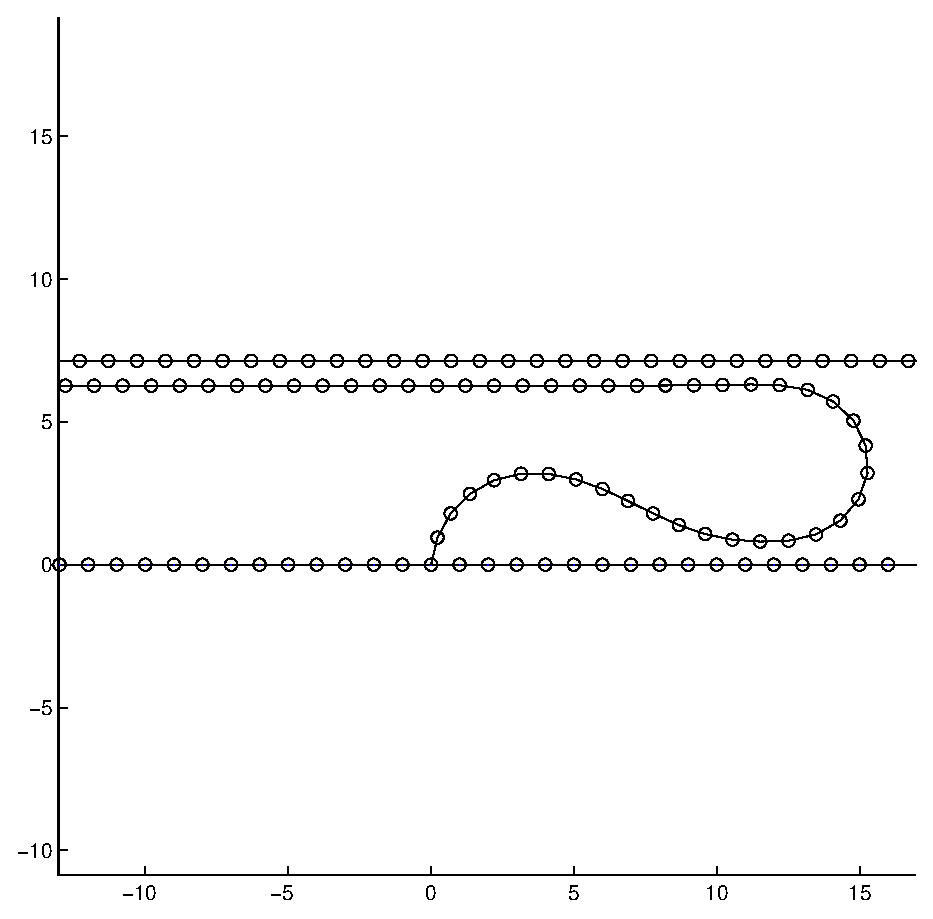
\includegraphics[scale=.4]{./fig/sims/push_b100/low_mag.eps}
			\caption{TODO \label{subfig:push_b100_low_mag}}
		\end{subfigure}%
		~
		\begin{subfigure}{.5\textwidth}
			\centering
			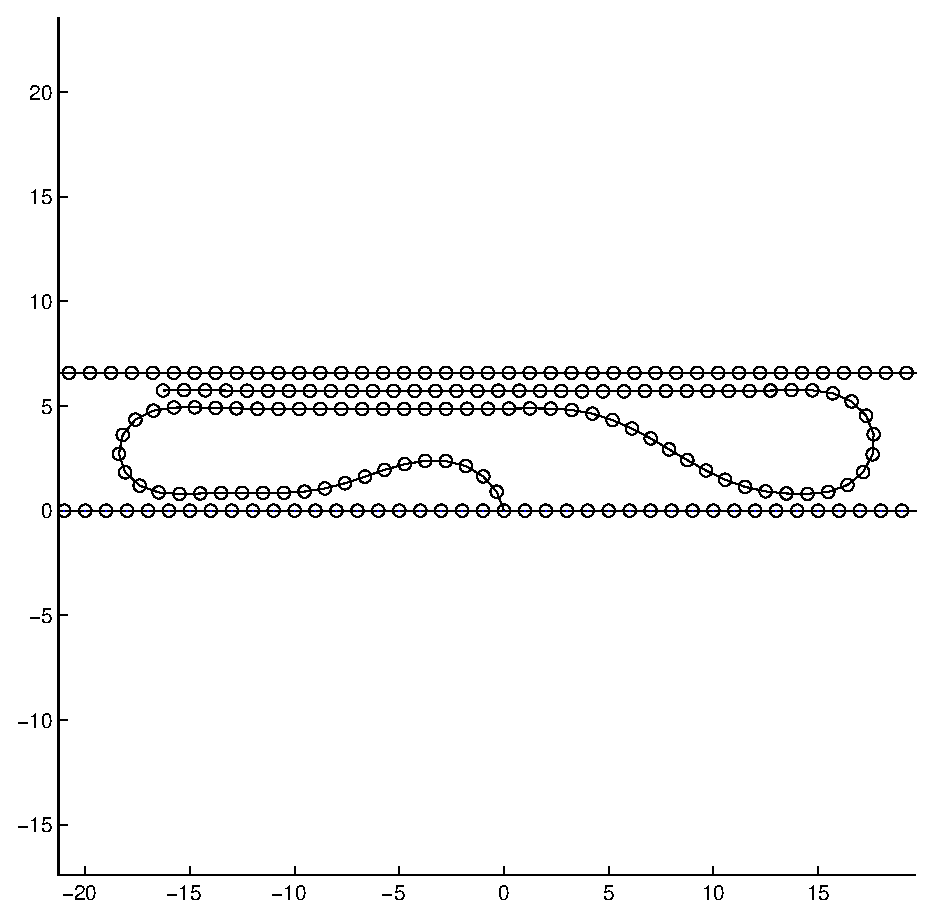
\includegraphics[scale=.4]{./fig/sims/push_b100/high_mag.eps}
			\caption{TODO \label{subfig:push_b100_high_mag}}
		\end{subfigure}

		\begin{subfigure}{.5\textwidth}
			\centering
			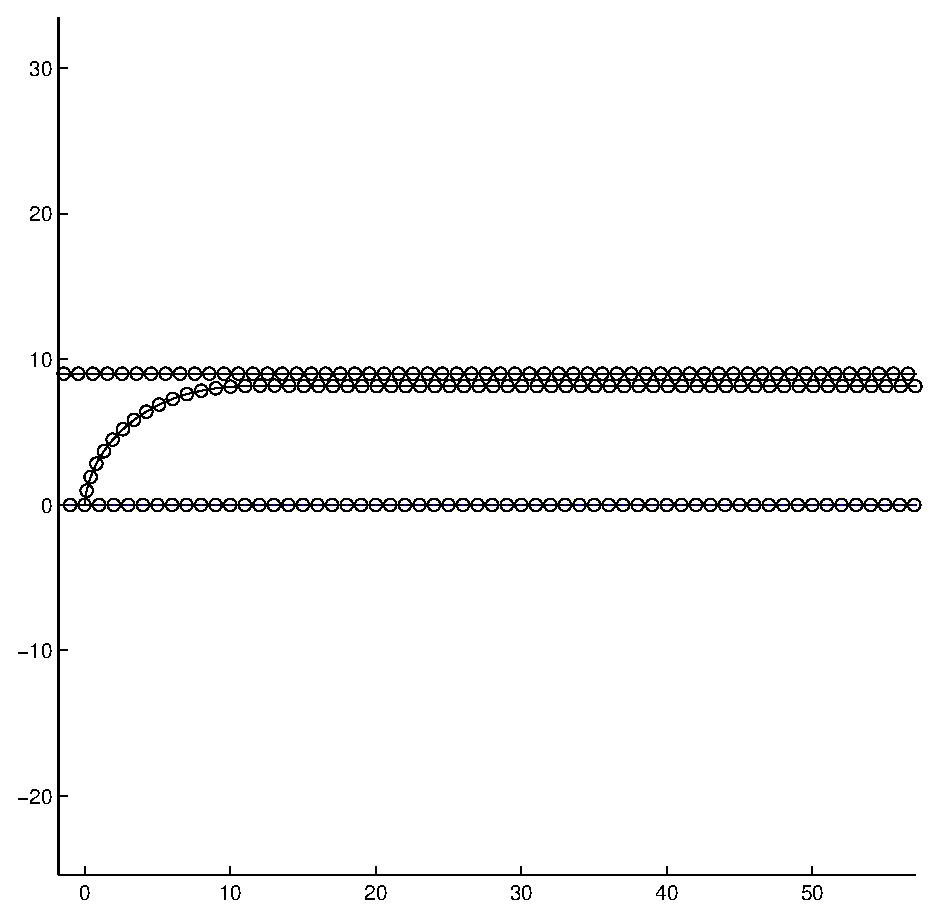
\includegraphics[scale=.4]{./fig/sims/push_b1000/bend.eps}
			\caption{TODO \label{subfig:push_b1000_bend}}
		\end{subfigure}		
		\caption{TODO\label{fig:push_bending}}	
	\end{figure*}

\subsection{Observations Increasing $\beta$}

Increasing $\beta$ shows a shrinking region for folding fibers under any load in Figure~\ref{fig:PushGrid:b100} and Figure~\ref{fig:PushGrid:b1000}. This suggests that folding in a fiber is a relation between $\beta$ and van der Waals (i.e. $\eps$ and $\eps^+$). The explanation being that folds can only occur when the top substrate is not causing the fiber to zip, either by load or overpowering van der Waals, and when $\beta$ is weak enough. If $\beta$ is strong enough to prevent folding it would suggest that the torsional springs are breaking crystallization with the top substrate as it compresses the fiber to shift more particles against the top substrate. As $\beta$ increases it would then become strong enough to break increasingly more crystallized particles with the top substrate to prevent a fold. Figure~\ref{subfig:push_b100_low_mag} and Figure~\ref{subfig:push_b100_high_mag} show configurations of different magnitude at $\beta = 10$ and how folds can still occur. Figure~\ref{subfig:push_b1000_bend} shows a configuration where no folding occurs. We also see that sufficiently strong $\beta$ and sufficiently weak magnitude of the load prevent a flattened configuration. We would expect the number of particles on the fiber that adhere to the top substrate to reduce if we continued to increase $\beta$. 

	\begin{figure}
		\begin{center}
			\includegraphics[scale=.5]{./fig/sims/push_eb0.1/p.eps}
		\end{center}		
		\caption{ TODO
		\label{fig:PushGrid:eb0.1}}
	\end{figure}	

	\begin{figure}
		\begin{center}
			\includegraphics[scale=.5]{./fig/sims/push_et0.1/p.eps}
		\end{center}		
		\caption{ TODO
		\label{fig:PushGrid:et0.1}}
	\end{figure}
	
	\begin{figure}
		\begin{center}
			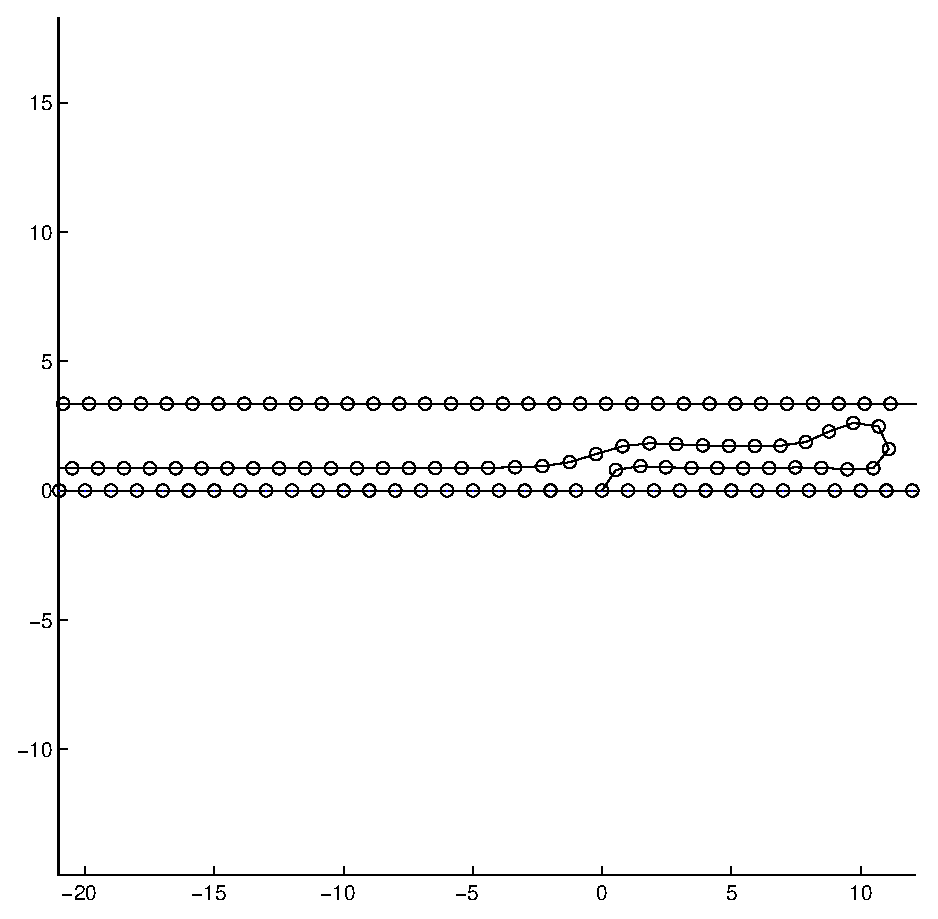
\includegraphics[scale=.4]{./fig/sims/push_et0.1/hump.eps}
		\end{center}		
		\caption{ TODO
		\label{fig:push_hump}}
	\end{figure}	

	\begin{figure}
		\begin{center}
			\includegraphics[scale=.5]{./fig/sims/push_eb0.1_et0.1/p.eps}
		\end{center}		
		\caption{ TODO
		\label{fig:PushGrid:eb0.1_et0.1}}
	\end{figure}	

	\begin{figure*}
		\centering
		\begin{subfigure}{.5\textwidth}
			\centering
			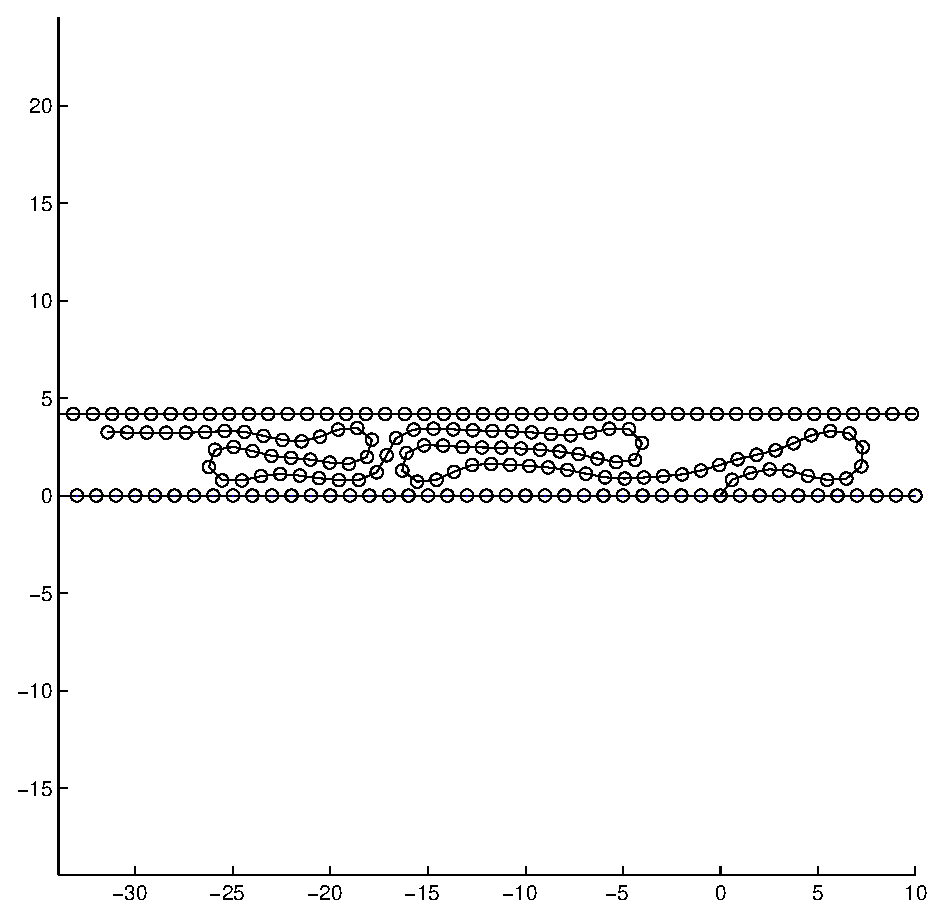
\includegraphics[scale=.4]{./fig/sims/push_eb0.1_et0.1/crumple.eps}
			\caption{TODO \label{subfig:push_crumple}}
		\end{subfigure}%
		~
		\begin{subfigure}{.5\textwidth}
			\centering
			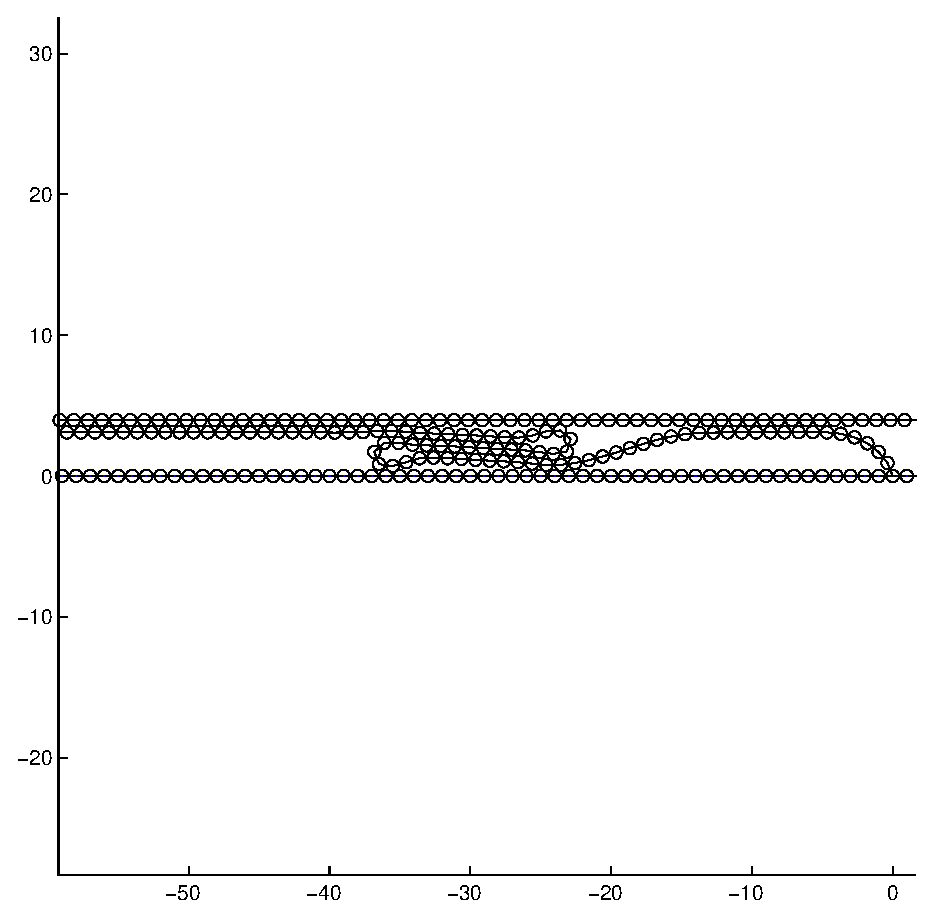
\includegraphics[scale=.4]{./fig/sims/push_eb0.1_et0.1/crumple2.eps}
			\caption{TODO \label{subfig:push_crumple2}}
		\end{subfigure}

		\begin{subfigure}{.5\textwidth}
			\centering
			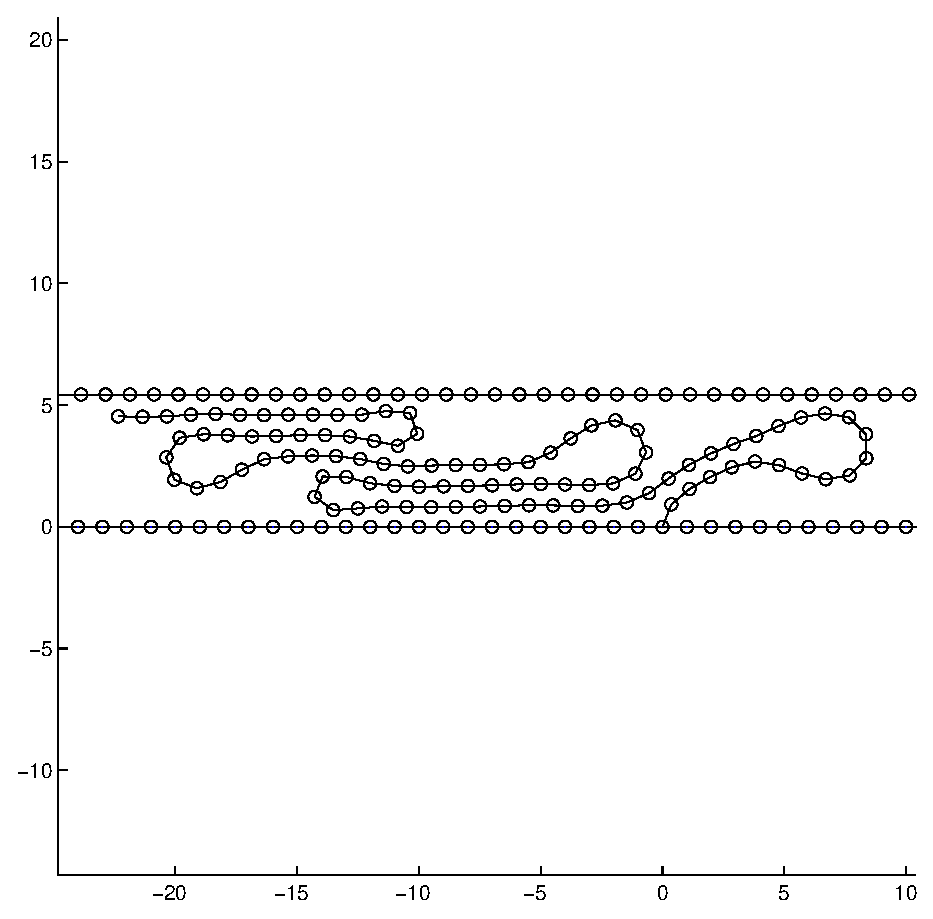
\includegraphics[scale=.4]{./fig/sims/push_eb0.1_et0.1/crumple3.eps}
			\caption{TODO \label{subfig:push_crumple3}}
		\end{subfigure}		
		\caption{TODO\label{fig:push_crumple}}	
	\end{figure*}

\subsection{Observations Decreasing $\eps^-$ and $\eps^+$} \label{subsection:push:eps}

An order of magnitude decrease in $\eps^-$ seems to play no qualitative role in equilibrium configurations, at least with the selected reference parameters (see Figure~\ref{fig:PushGrid:eb0.1}). However, an order of magnitude decrease in $\eps^+$ plays a significant role (see Figure~\ref{fig:PushGrid:et0.1}). The shear component of the load instead of causing the fiber to zip to the top substrate causes the top substrate to slide off. That is, the van der Waals interaction is not strong enough for large shear components or large magnitudes to hold or adhere to the fiber. Even so and angled load is necessary to cause a flattened configuration, but the region of angles that cause folding as increased. This is because with sufficiently small shear component will cause the fiber to buckle and then van der Waals interaction between particles on the fiber will be the dominate force as the fiber zips against itself. The isolated white regions of Figure~\ref{fig:PushGrid:et0.1} are of a ``hump'' configuration (see Figure~\ref{fig:push_hump}). The hump is caused by the fiber zipping to the bottom substrate with fold immediately at the root causing a ``hump''. The top substrate is then only adhered to a single particle of the fiber. If both $\eps^-$ and $\eps^+$ are decreased by an order of magnitude then we have a similar diagram as with only $\eps^-$ being reduced but the ``hump'' configuration is lost (see Figure~\ref{fig:PushGrid:eb0.1_et0.1}). This variation from the reference parameters weakens adhesion of all van der Waals interactions between the fiber and either substrate but keeps the same interaction between particles on the fiber with other particles on the fiber. Therefore, folding is more prominent for the same reasons that folding was more prominent when only $\eps^-$ was decreased.
	
	\begin{figure}
		\begin{center}
			\includegraphics[scale=.5]{./fig/sims/push_g1000/p.eps}
		\end{center}		
		\caption{ TODO
		\label{fig:PushGrid:g1000}}
	\end{figure}	

\subsection{Observations Increasing $\gamma$}

An order of magnitude increase in $\gamma$ has no observable effect (see Figure~\ref{fig:PushGrid:g1000}). The purpose of $\gamma$ is to keep the particles a fixed distance apart but allow for some relaxation. If $\gamma$ were very large we might expect the bonds to be too stiff and prevent crystallization. However, the uniform spacing between particles on the substrates and the ideal spacing, $\ell$, of particles on the fiber allow for at least some crystallization regardless of how stiff the extensible spring is made to be. Intuitively, it would seem that even with very stiff extensible springs the diagram would still not vary significantly from Figure~\ref{fig:PullGrid}.

	\begin{figure}
		\begin{center}
			\includegraphics[scale=.5]{./fig/sims/push_p1_oscount0/p.eps}
		\end{center}		
		\caption{ TODO
		\label{fig:PushGrid:p1}}
	\end{figure}

\subsection{Replacing Atomized Bottom Substrate with Pressure}

Up until now all experiments have been done with a bottom substrate comprised of contiguous particles. However, varying the van der Waals strength of these particles with particles of the fiber didn't have any qualitative effect as shown in Subsection~\ref{subsection:push:eps}. We might ask if particles on the bottom substrate are necessary at all to the behavior of the fiber. Thus, we remove all particles on the bottom substrate and replace the van der Waals interaction with a pressure (see Figure~\ref{fig:PushGrid:p1}. \textbf{TODO}(introduce the equation here? In Chapter 2?) We can see some general similarities between the reference diagram and a bottom substrate replaced with pressure. However, there are also some noticeable anomalies. There are ``hump'' like configurations and different folding behavior. \textbf{TODO}(I don't have an explanation)

%How the fiber deforms under compression, in particular the amount of the fiber under contact, is a question that has been asked and answered in other contexts
\textbf{TODO}(Cite Majidi and He).

\section{Detachment}

	\begin{table}
		\rowcolors{1}{}{lightgray}
		\centering
		\caption{Reference parameters for compression. \label{table:detachment_reference}}
		\begin{tabular}{lcrclcr}
			$m$ & = & 1 & \hspace{1in} & $\ell_-$ & = & 1 \\
			$n$ & = & 96 & & $\ell_+$ & = & 1 \\
			$n_+$ & = & 300 & & $\ell$ & = & 1 \\
			$n_-$ & = & 300 & & $\gamma$ & = & 100 \\
			$x^{(-)}$ & = & -150 & & $\beta$ & = & 1 \\
			$y^{(-)}$ & = & 0 & & $\eps^-$ & = & 1 \\
			$x^{(+)}$ & = & -150 & & $\eps^+$ & = & 1 \\
			$y^{(+)}$ & $\approx$ & 1.72741 & & $\eps$ & = & 1 \\
			$\delta$ & = & 0 & & $\sigma$ & = & 1
		\end{tabular}
	\end{table}
	
	\begin{figure}[h]
		\begin{center}
			\includegraphics[scale=.5]{./fig/sims/pull/p.eps}
		\end{center}		
		\caption{ TODO
		\label{fig:PullGrid}}
	\end{figure}
	
	\begin{figure}[h]
		\begin{center}
			\includegraphics[scale=.5]{./fig/sims/pull_b10/p.eps}
		\end{center}		
		\caption{ TODO
		\label{fig:PullGrid:b10}}
	\end{figure}
	
	\begin{figure}[h]
		\begin{center}
			\includegraphics[scale=.5]{./fig/sims/pull_b100/p.eps}
		\end{center}		
		\caption{ TODO
		\label{fig:PullGrid:b100}}
	\end{figure}
	
	\begin{figure}[h]
		\begin{center}
			\includegraphics[scale=.5]{./fig/sims/pull_eb0.1/p.eps}
		\end{center}		
		\caption{ TODO
		\label{fig:PullGrid:eb0.1}}
	\end{figure}

	\begin{figure}[h]
		\begin{center}
			\includegraphics[scale=.5]{./fig/sims/pull_eb0.01/p.eps}
		\end{center}		
		\caption{ TODO
		\label{fig:PullGrid:eb0.01}}
	\end{figure}
	
	\begin{figure}[h]
		\begin{center}
			\includegraphics[scale=.5]{./fig/sims/pull_eb0/p.eps}
		\end{center}		
		\caption{ TODO
		\label{fig:PullGrid:eb0}}
	\end{figure}
	
	\begin{figure}[h]
		\begin{center}
			\includegraphics[scale=.5]{./fig/sims/pull_eb0.1_et0.1/p.eps}
		\end{center}		
		\caption{ TODO
		\label{fig:PullGrid:eb0.1_et0.1}}
	\end{figure}
	
	\begin{figure}[h]
		\begin{center}
			\includegraphics[scale=.5]{./fig/sims/pull_eb0.1_et0.1_e0.1/p.eps}
		\end{center}		
		\caption{ TODO
		\label{fig:PullGrid:eb0.1_et0.1_e0.1}}
	\end{figure}
	
	\begin{figure}[h]
		\begin{center}
			\includegraphics[scale=.5]{./fig/sims/pull_et10/p.eps}
		\end{center}		
		\caption{ TODO
		\label{fig:PullGrid:et10}}
	\end{figure}
	
	\begin{figure}[h]
		\begin{center}
			\includegraphics[scale=.5]{./fig/sims/pull_g1000/p.eps}
		\end{center}		
		\caption{ TODO
		\label{fig:PullGrid:g1000}}
	\end{figure}
	
	\begin{figure}[h]
		\begin{center}
			\includegraphics[scale=.5]{./fig/sims/pull_p1_oscount0/p.eps}
		\end{center}		
		\caption{ TODO
		\label{fig:PullGrid:p1}}
	\end{figure}
	
	\begin{figure}[h]
		\begin{center}
			\includegraphics[scale=.5]{./fig/sims/pull_p10_oscount0/p.eps}
		\end{center}		
		\caption{ TODO
		\label{fig:PullGrid:p10}}
	\end{figure}


\subsection{Observations of Reference Parameters}

\subsection{Observations Increasing $\beta$}

\subsection{Observations Decreasing $\eps^-$}

\subsection{Observations Decreasing $\eps^-$, $\eps^+$, and $\eps$}

\subsection{Observations Increasing $\eps^+$}

\subsection{Observations Increasing $\gamma$}

\subsection{Replacing Atomized Bottom Substrate with Pressure}




\section{Conclusions}
\chapter{Many fiber simulations} \label{chap:four}

\section{Proof of concept}

	\begin{table}
		\rowcolors{1}{}{lightgray}
		\centering
		\caption{Reference parameters for all simulations presented in this chapter. Note that $n_j$ and $\delta_j$ are functions of $j$. For each $j$, $n_j$ is constant and $\delta_j$ is linear. \label{table:manyfiber_reference}}
		\begin{tabular}{lcrclcr}
			$m$ & = & 10 & \hspace{1in} & $\ell_-$ & = & 1 \\
			$n_j$ & = & 96 & & $\ell_+$ & = & 1 \\
			$n_+$ & = & 360 & & $\ell$ & = & 1 \\
			$n_-$ & = & 310 & & $\gamma$ & = & 100 \\
			$x^{(-)}$ & = & -110 & & $\beta$ & = & 10 \\
			$y^{(-)}$ & = & 0 & & $\eps_-$ & = & 0.1 \\
			$x^{(+)}$ & = & -160 & & $\eps_+$ & = & 1 \\
			$y^{(+)}$ & = & 110 & & $\eps$ & = & 0.1 \\
			$\delta_j$ & = & 10$j$ & & $\sigma$ & = & 1
		\end{tabular}
	\end{table}

	In Chapter~\ref{chap:three} we discussed three different simulation experiments. Here we look at the compression experiment with ten fibers. As before we have a set of reference parameters (see Table~\ref{table:manyfiber_reference}). We run the compression experiment for the reference parameters and three variations of the parameters, specifically varying $\beta$, $\gamma$, and $\eps_+$.

	\begin{figure}
		\begin{center}
			\includegraphics[scale=1]{./fig/ch4/grid.eps}
		\end{center}		
		\caption{Equilibrium configurations of ten fibers with 96 particles each for varying loads. The top left plot is a configuration with a load of $\lambda = 5$ and $\mu = 0$. The configurations to the right and below correspond to an increasing $\mu$ and increasing $\lambda$ respectively. All configurations use the reference parameters in Table~\ref{table:manyfiber_reference}.
		\label{fig:grid}}
	\end{figure}
	
	We consider nine simulations with values of $\lambda = 5, 15, 25$ and $\mu = 0, 5, 10$. In Figure~\ref{fig:grid} we see a high level view of each simulation for the reference parameters. Keeping the horizontal component of the load zero, we see an increase in bends of all ten fibers as we increase $\lambda$. One explanation for this is that the torsional and extensible springs do not have enough time to slide along the top substrate and align to it. As the magnitude of the vertical component of the load is increased the fibers become more likely to buckle. 
	
	If we increase the horizontal component of the load the story changes. We are able to maintain the aligned compressed configuration for larger magnitudes of the load if the horizontal component is sufficiently large. It would seem that the ratio between vertical and horizontal component for the reference parameters is the deciding factor for whether or not fibers will buckle. This is analogous to crushed configurations for $\theta$ near $0$\textdegree\ and flattened configurations for increased $\theta$ in Chapter~\ref{chap:three} 

	\begin{figure}
		\begin{center}
			\includegraphics[scale=1]{./fig/ch4/grid_b100.eps}
		\end{center}		
		\caption{Equilibrium configurations of varying loads. All configurations are directly comparable to Figure~\ref{fig:grid} with the exception that $\beta = 100$.
		\label{fig:grid_b100}}
	\end{figure}

	In Figure~\ref{fig:grid_b100} we increase $\beta$ to one hundred. This is an order of magnitude increase from the reference parameters and it prevents buckling at all selected loads. Qualitatively there is no discernible difference in any of the nine simulations with the one exception that the fibers buckle to the left with no horizontal component of the load. The ``crushed'' configurations of the reference parameters no longer occur similar to the single fiber situation. Although the single bend of a fiber for a single fiber only occured for $\beta=1000$ perhaps the inter-fiber vdW interaction reinforces this configuration.
	
	\begin{figure}
		\begin{center}
			\includegraphics[scale=1]{./fig/ch4/grid_g1000.eps}
		\end{center}		
		\caption{Equilibrium configurations of varying loads. All configurations are directly comparable to Figure~\ref{fig:grid} with the exception that $\gamma = 1000$.
		\label{fig:grid_g1000}}
	\end{figure}
	
	We observe that the increase in the torsional spring strength prevents buckling to happen anywhere except the junction between the fiber and the substrate. On the other hand when we increase the extensible spring constant by an order of magnitude the buckling patterns are the same as those observed for the reference parameters. Comparing Figure~\ref{fig:grid_g1000} to Figure~\ref{fig:grid}, the same kinds of configurations are present in both. With $\gamma$ sufficiently large and vdW sufficiently weak, further increasing $\gamma$ plays a negligible role because the distance between particles on a fiber is already close to $\ell$.
	
	\begin{figure}
		\begin{center}
			\includegraphics[scale=1]{./fig/ch4/grid_et0.1.eps}
		\end{center}		
		\caption{Equilibrium configurations of varying loads. All configurations are directly comparable to Figure~\ref{fig:grid} with the exception that $\eps_+ = 0.1$.
		\label{fig:grid_et0.1}}
	\end{figure}

	Next, consider the situation when all vdW strengths in the system are the same. In Figure~\ref{fig:grid_et0.1} we reduce $\eps_+$ to 0.1 and present the results for nine different loads while keeping the rest of the parameters equal to the reference values. For $\mu = 0$ or $5$ the configurations are comparable. We further observe that the horizontal component of the load can be strong enough to cause the top substrate to slide off the fibers overpowering the vdW interaction. This happens for all values of the vertical component of the load that we have considered when $\mu = 10$.
	
	Although we focus primarily on the model for only a single fiber it was designed for arbitrarily many and arbitrarily large fibers. Investigating the single fiber case does give us some insight into how many fibers will behave as well.

\section{Future work}

The single fiber scenario presented in Chapter~\ref{chap:three} varied two parameters for each plot.
This approach gave interesting results for the specific parameters of interest ($\lambda$ and $\mu$) but it does not as effectively explore the rest of the parameter space.
Likewise, many of the arguments for the behavior of the system are either by direct example or from numerical trends of the simulations.
There are four modes of detachment discovered, simple sliding, wave propagated sliding, brute forcing, and unzipping.
It appears that are only really two modes of detachment, sliding and unzipping, but this is not entirely clear from numerical experiment alone.

For many fibers it is more difficult to explore the parameter space in a way to categorize exact equilibrium configurations simply because of the number of particles.
However, a sensitivity analysis of the parameter space could give insight into the behavior and a detachment experiment with many fibers would demonstrate how the detachment modes behave with inter-fiber adhesion.
Applying the model to physical situations is out of the scope of this work but parameterization of ``bead-spring'' models of similar kind have been used to some success to model CNTs.


\bibliographystyle{ieeetr}
\bibliography{bio}
%If you have n appendices, then use the \appendices{n} command below
%followed by n \input{filename} commands, similar to the \input{chapx}
%commands above.
% DO NOT USE SECTIONS OR SUBSECTIONS IN AN APPENDIX OR APPENDICES
\appendix{2}
%\chapter{Introduction to CUDA} \label{ap:a}


CUDA is a propriety architecture developed by nVIDIA. The purpose of CUDA is to pioneer the concept of general purpose graphical processing units (GPGPUs). CUDA offers an interface and structure to abstract away the hardware of nVIDIA GPU architectures in order for a programmer to more readily developed for a GPU. The benefit of a parallel speed up is quite obvious for any application with sufficient throughput potential.

That is, if we imagine the CPU has one capable and intricate shoveller, then the GPU can be visualized as hundreds or even thousands of very dumb shovellers. It is not hard from this analogy to gain insight into many advantages and disadvantages on both architectures. For instance, the CPU is much better at tasks that are interdependent or require a complex control structure, the smart shoveller is capable of handling and remembering complicated sequences of tasks that are conditional dependent on prior ones. In contrast, the GPU is significantly better at simplified tasks. If the programmer can accurately express her problem in terms of a sequence of non-conditional dependent tasks, then a dumb shoveller will be able to remember and executed those tasks in a timely fashion.

Imagine the task where either the CPU or the GPU must recreate a piece of artwork out of varying levels of indentation into a plot of land. The GPU, or many dumb shovellers, will simply get in each others way. Imagine the task where either the CPU or the GPU must level out a plot of land. Each dumb shoveller need only be allocated part of the plot and dig a flat surface to the predetermined depth, each can perform this task simultaneously. The larger the plot of land, the better the GPU will perform in comparison.

However, there is still a level of management that is expected of the programmer. These ones simple tasks can become quite complicated when you are management thousands of shovellers.



\chapter{MATLAB code} \label{ap:b}

\lstset{
	language=Matlab,
	basicstyle=\scriptsize,
	tabsize=2,
	breaklines=true,
	breakatwhitespace=true
}

\singlespacing

\lstinputlisting{matlab_code/force.m}

\chapter{C++ code} \label{ap:c}

\lstset{
	language=C++,
	basicstyle=\footnotesize,
	tabsize=2,
	breaklines=true,
	breakatwhitespace=true
}

\singlespacing

\lstinputlisting{code/defs.h}

\lstinputlisting{code/parameter.h}

\lstinputlisting{code/serial/force.h}

\lstinputlisting{code/serial/force.cpp}

\lstinputlisting{code/main.cpp}

\lstinputlisting{code/json/JSON_checker.h}

\lstinputlisting{code/json/JSON_checker.cpp}

\lstinputlisting{code/json/json.h}

\lstinputlisting{code/json/json.cpp}

\lstinputlisting{code/CMakeLists.txt}

\end{document}
